\documentclass[12pt,a4paper]{book}
\special{papersize=210mm,297mm}
\usepackage[T1]{fontenc}
\usepackage[utf8]{inputenc}
\usepackage[spanish]{babel}
\usepackage{csquotes}
\usepackage{graphicx}
\usepackage[hidelinks]{hyperref}
\usepackage[acronym]{glossaries}
\usepackage[style=ieee, backend=bibtex,
natbib=true, language=spanish]{biblatex}
\usepackage{sectsty}
\usepackage{tikz}
\usetikzlibrary{babel}
\usetikzlibrary{positioning}
\usetikzlibrary{arrows, arrows.meta}
\allsectionsfont{\raggedright}
\urlstyle{same}
\renewbibmacro{in:}{}
\DeclareFieldFormat*{title}{"#1"}
\DeclareFieldFormat*{citetitle}{#1}
\DefineBibliographyStrings{spanish}
{
  url = {Dirección},
  presentedat = {presentado en }
}
\addbibresource{biblio.bib}
\graphicspath{ {./images/} }
\makenoidxglossaries
\renewcommand{\glsnamefont}[1]{\makefirstuc{#1}}
\newacronym{unam}{UNaM}{Universidad Nacional de Misiones}
\newacronym{fceqyn}{FCEQyN}{Facultad de Ciencias Exactas, Químicas y Naturales}
\newacronym{lsi}{Lic. en Sist. de Información}{Licenciatura en Sistemas de Información}
\newacronym{pylp}{Paradigmas y Leng. de Prog.}{Paradigmas y Lenguajes de Programación}
\newacronym{gnu}{GNU}{GNU's Not Unix}
\newacronym{gnome}{GNOME}{GNU Network Object Model Environment}
\newacronym{kde}{KDE}{K Desktop Environment}
\newacronym{xfce}{Xfce}{X Free Cholesterol Environment}
\newacronym{lxqt}{LXQt}{Lightweight X11 Qt}
\newacronym{vmm}{virt-manager}{Virtual Machine Manager}
\newacronym{mv}{MV}{Máquina Virtual}
\newacronym{so}{SO}{Sistema Operativo}
\newacronym{cpu}{CPU}{Central Processing Unit}
\newacronym{gdm}{GDM}{GNOME Display Manager}
\newacronym{ghc}{GHC}{GNU Haskell Compiler}
\newacronym{tui}{TUI}{Terminal User Interface}
\newglossaryentry{de}
{
  name={entorno de escritorio},
  plural={entornos de escritorio},
  description={Conjunto de software para ofrecer al usuario de
  una computadora una interacción amigable y cómoda. Es una
  implementación de interfaz gráfica de usuario que ofrece
  facilidades de acceso y configuración, como barras de
  herramientas e integración entre aplicaciones con habilidades
  como arrastrar y soltar}
}
\newglossaryentry{wm}
{
  name={gestor de ventanas},
  plural={gestores de ventanas},
  description={Programa informático que controla la
  ubicación y apariencia de las ventanas bajo un
  sistema de ventanas en una interfaz gráfica de usuario}
}
\newglossaryentry{comp}
{
  name={compositor de ventanas},
  plural={compositores de ventanas},
  description={Componente de la interfaz gráfica de una
  computadora que dibuja las ventanas o sus bordes. Éste
  también controla cómo éstas son mostradas y cómo
  interactúan con otras ventanas y el resto del entorno
  del escritorio}
}
\newglossaryentry{serv}
{
  name={servidor de ventanas},
  plural={servidores de ventanas},
  description={Programa cuya tarea principal es coordinar
  la entrada y la salida de sus clientes hacia y desde el
  resto del sistema operativo, el hardware, y otros. El
  servidor gráfico se comunica con sus clientes con el
  protocolo de servidor gráfico}
}

\begin{document}
	\frontmatter
	\pagenumbering{gobble}
	\begin{center}
	{\fontsize{30pt}{36pt}\selectfont
	\textbf{Trabajo Final}}
	\newline
	\large{Entorno de escritorio con
	gestor de ventanas XMonad en Haskell}
	\newline
\end{center}
\huge{\underline{Universidad:} \acrshort{unam}}
\vspace{36pt}
\newline
\huge{\underline{Facultad:} \acrshort{fceqyn}}
\vspace{36pt}
\newline
\huge{\underline{Carrera:} \acrshort{lsi}}
\vspace{36pt}
\newline
\huge{\underline{Cátedra:} \acrshort{pylp}}
\vspace{36pt}
\newline
\huge{\underline{Alumno:} Antoniak, Rodrigo Lionel}
\vspace{36pt}
\newline
\huge{\underline{Profesores:}}
\newline
\huge{Pautsch, Germán}
\newline
\huge{Martini, Esteban}
\vspace{36pt}
\newline
\huge{\underline{Año:} 2022}

	\cleardoublepage
	\pagestyle{plain}
	\pagenumbering{Roman}
	\setcounter{page}{3}
	\tableofcontents
	\listoftables
	\listoffigures
	\cleardoublepage
	\mainmatter
	\pagestyle{headings}
	\pagenumbering{arabic}
	\setcounter{page}{5}
	\part{Introducción}
	\normalsize{ \indent
Este trabajo práctico final se ha realizado
con el objetivo de completar la cátedra de
\acrlong{pylp} (en el año 2022), perteneciendo
a la carrera de \acrlong{lsi}; correspondiente
a la \acrlong{fceqyn}, que ofrece la \acrlong{unam}.
}
\newline
\normalsize{ \indent
En él, se desarrolla una implementación de un \Gls{de}
desde el gestor de ventanas XMonad \cite{haskell_xmonad};
donde cada ventana se encuentra en mosaicos y está
escrito en el lenguaje Haskell. En conjunto, se utiliza
la barra de estado XMobar \cite{hackage_xmobar}, el
emulador de terminal Termonad \cite{hackage_termonad}, el
lanzador de aplicaciones Rofi \cite{rofi} y una aplicación
para gestionar una sesión activa (con acciones como apagar,
reiniciar y cerrar sesión).
}

	\part{Desarrollo}
	\chapter{Justificación}
	\normalsize{ \indent
En la actualidad, todas las computadoras personales utilizan
una interfaz gráfica para interactuar con el usuario. Más
allá del sistema operativo que se utilice, el entorno visual
que se utilice en el espacio personal es esencial; tomando en
cuenta la facilidad de uso, comodidad y personalización, entre
otros aspectos.
}
\newline
\normalsize{ \indent
Dependiendo de la arquitectura del sistema operativo, podrán
existir distintas opciones para los entornos de escritorio de
la computadora personal. En el caso de Windows \cite{dwm_exe},
el motor gráfico está definido a nivel del kernel (como se
muestra en
\url{https://learn.microsoft.com/es-ar/windows-hardware/drivers/display/images/dpy1.png} y
\url{https://en.wikipedia.org/wiki/Architecture_of_Windows_NT#/media/File:Windows_2000_architecture.svg});
esto limita a que deba utilizarse el entorno gráfico que define
Microsoft para su sistema operativo. En cambio, los sistemas
operativos basados en UNIX \cite{x_wayland} pueden elegir su
propio entorno de escritorio (por lo tanto, su gestor de
ventanas) porque su arquitectura en capas lo permite.
}
\newline
\normalsize{ \indent
A continuación, se mostrará cómo se gestiona el entorno gráfico
en un sistema operativo Linux para computadoras personales (se
aclara esto porque los servidores no cuentan normalmente con
ninguna interfaz gráfica por defecto):
}
\newline
\begin{tikzpicture}[
  cuadro/.style={rectangle, draw=black!50, fill=white!3,
  very thick, minimum size=3mm},
]
  \node[cuadro] (usuario) {Usuario};
  \node[cuadro] (gui) [below=of usuario] {\Gls{de}};
  \node[cuadro] (ventanas) [below=of gui] {\Gls{wm}};
  \node[cuadro] (servidor) [below=of ventanas] {\Gls{serv}};
  \node[cuadro] (compositor) [right=of servidor] {\Gls{comp}};
  \node[cuadro] (kernel) [below=of servidor] {Núcleo};
  \node[cuadro] (hw) [below=of kernel] {Hardware};
  \draw[>=triangle 45, <->] (usuario.south) -- (gui.north);
  \draw[>=triangle 45, <->] (gui.south) -- (ventanas.north);
  \draw[>=triangle 45, <->] (ventanas.south) -- (servidor.north);
  \draw[>=triangle 45, <->] (servidor.south) -- (kernel.north);
  \draw[>=triangle 45, <->] (kernel.south) -- (hw.north);
  \draw[>=triangle 45, <->] (servidor.east) -- (compositor.west);
\end{tikzpicture}
\newline
\normalsize{ \indent
Un ejemplo de entorno gráfico completo para el esquema
anteriormente mostrado es el siguiente:
}
\begin{itemize}
  \setlength\itemsep{1pt}
  \item \Gls{serv}: X.Org.
  \item \Gls{comp}: picom.
  \item \Gls{wm}: xfwm4.
  \item \Gls{de}: \acrshort{xfce}.
\end{itemize}
\ \newline
\normalsize{ \indent
En la actualidad, existe una gran cantidad de entornos
de escritorio para \acrshort{gnu}/Linux; desde
\acrshort{gnome} y \acrshort{kde}, hasta \acrshort{xfce},
\acrshort{lxqt} y otros. Cada uno de ellos se caracteriza
por su aspecto, conjunto de herramientas y gestor de
ventanas; además de características comparables entre sí,
como el consumo eléctrico y de memoria.
}
\newline
\normalsize{ \indent
Más allá de los pros y contras que posee cada uno de
los anteriormente citados, todos comparten la propiedad
de ser muy conducidos al uso del ratón o pad táctil. Sin
embargo, el usuario puede decidir por interactuar
directamente con el gestor de ventanas; en consecuencia,
la cantidad de capas que interviene en la interacción
humano-computadora es menor y se favorece al menor
consumo de recursos.
}
\newline
\normalsize{ \indent
Además, debe considerarse la salud de las manos con el
uso del ratón \cite{desorden_extremidades}; donde existen
estudios que demuestran los efectos negativos del mouse
promedio \cite{dermatosis}. A pesar de la existencia de
ratones ergonómicos \cite{hipotermia_munieca}, estos
últimos son personales; cada uno se adapta a un tamaño
particular de mano, incluyendo el hecho de haber varias
formas ergonómicas y un costo económico elevado.
}
\newline
\normalsize{ \indent
Por lo tanto, se puede concretar que la utilización
de un gestor de ventanas en mosaico es factible por
varias razones; algunas de las cuales son el consumo
de recursos y la disminución del uso del mouse, entre
otros (ciertas motivaciones son más enfocadas para
desarrolladores, como la programación y la
personalización; mientras que otras pueden observarse
como subjetivas, evitándose incluirse para mantener
la objetividad de la justificación).
}

	\chapter{Objetivos}
	\section[General]{Objetivo General}
\begin{itemize}
  \item Implementar un entorno de escritorio
  utilizable con XMonad \cite{haskell_xmonad}
  en Haskell.
\end{itemize}
\section[Específicos]{Objetivos Específicos}
\begin{itemize}
  \item Ajustar los atajos de teclado a gusto
  personal.
  \item Agregar un menú que se asemeje a la función
  del menú de inicio de Windows.
  \item Cambiar la barra de estado por defecto en
  XMonad (Polybar) por XMobar \cite{hackage_xmobar}.
  \item Reemplazar el emulador de terminal por
  defecto por Termonad \cite{hackage_termonad}.
  \item Personalizar la aplicación para salir
  de la sesión actual con Haskell.
\end{itemize}

	\chapter{Alcance}
	\normalsize{ \indent
En este trabajo, se abarcará la implantación del
gestor de ventanas en mosaico XMonad; en conjunto con
una configuración personalizada, la cual pueda satisfacer
la mayoría de necesidades de los usuarios en promedio.
Considerando que muchos usuarios utilizan entornos de
escritorio completos, se contempla las utilidades que
las personas generalmente necesitan a continuación:
}
\begin{itemize}
  \item Menú que permita acceder a las aplicaciones
  deseadas de un menú de inicio.
  \item Barra de estado que indica los parámetros
  actuales del sistema (XMobar).
  \item Accesibilidad hacia el control de los
  periféricos de la computadora, como la salida
  de sonido, WiFi, Bluetooth, almacenamiento
  extraíble, entre otros.
  \item Menú que permita realizar distintas
  acciones con la sesión activa, tales como apagar,
  reiniciar, cerrar sesión suspender, hibernar y
  dormir.
\end{itemize}
\ \newline
\normalsize{ \indent
No se pretende demostrar todas las capacidades que
posee XMonad, las cuales son varias; sino que se
alcanza hasta las funciones básicas requeridas para
la adaptación de un usuario, el cual está acostumbrado
a un entorno de escritorio completo.
}
\newline
\normalsize{ \indent
Para el lector que desee explorar las configuraciones
y personalizar su sistema al máximo, con objetivo de
lograr el entorno más cómodo y productivo para sí
mismo; se encomienda que busque obtener sus metas
personales por su cuenta, ya que los gestores de
ventanas en mosaico dan la posibilidad de ajustar el
escritorio a gusto de cada usuario.
}
\newline
\normalsize{ \indent
Adicionalmente, se utilizará el lanzador de aplicaciones
Rofi; en consecuencia, se podrá ejecutar programas sin
necesidad de personalizarlo en el menú de inicio. También,
se cambiará la terminal por defecto de la distribución
de Linux a seleccionar por Termonad; buscando mostrar las
capacidades del lenguaje de programación Haskell.
}

	\chapter{Recursos}
	\normalsize{ \indent
Para poder realizar lo propuesto, se ha utilizado una
máquina virtual; con objetivo de poder trasportar los
logros a distintas computadoras, además de evitar una
instalación fisica en hardware directamente. El
virtualizador que se ocupará es \acrshort{vmm},
considerando la facilidad que provee de personalización;
incluyendo características esenciales como traspaso de
dispositivos huésped y lector de discos, entre otros.
}
\newline
\normalsize{ \indent
Las características de los sistemas operativos
utilizados son:
}
\begin{figure}[!ht]
  \caption{Computadora huésped}
  \centering
  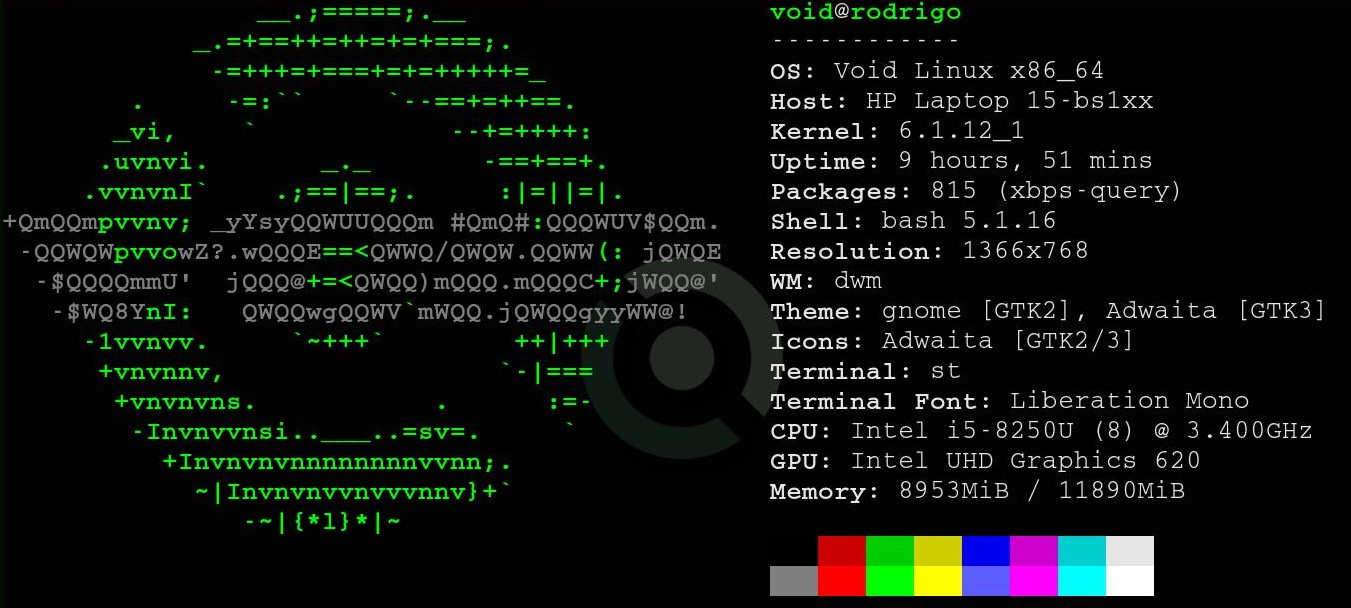
\includegraphics[width=\textwidth]{hostMachine}
\end{figure}
\begin{figure}[!ht]
  \caption{Máquina virtual}
  \centering
  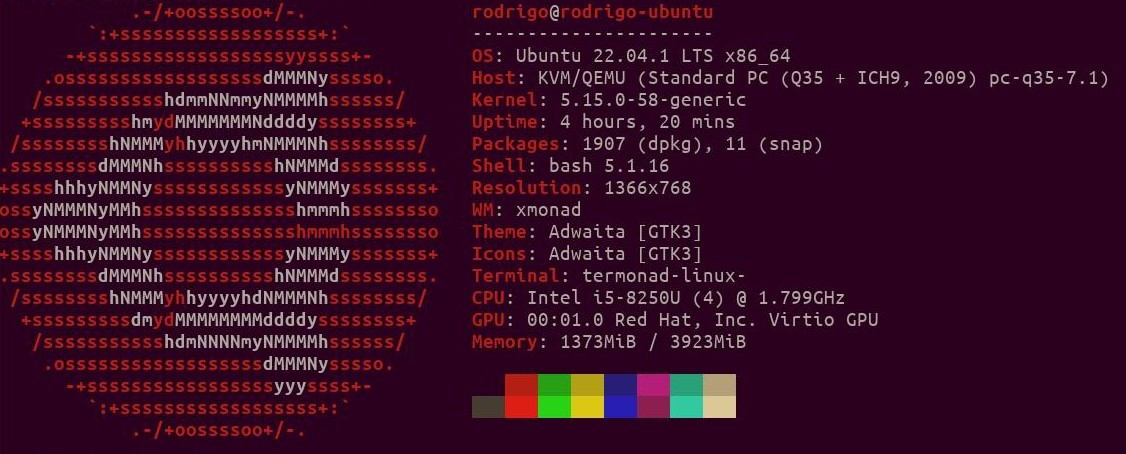
\includegraphics[width=\textwidth]{guestMachine}
\end{figure}
\newline
\normalsize{ \indent
La \acrlong{mv} se encuentra configurada de la
siguiente forma:
}
\newpage
\begin{figure}[!ht]
  \caption{Vistazo de \acrshort{mv}}
  \centering
  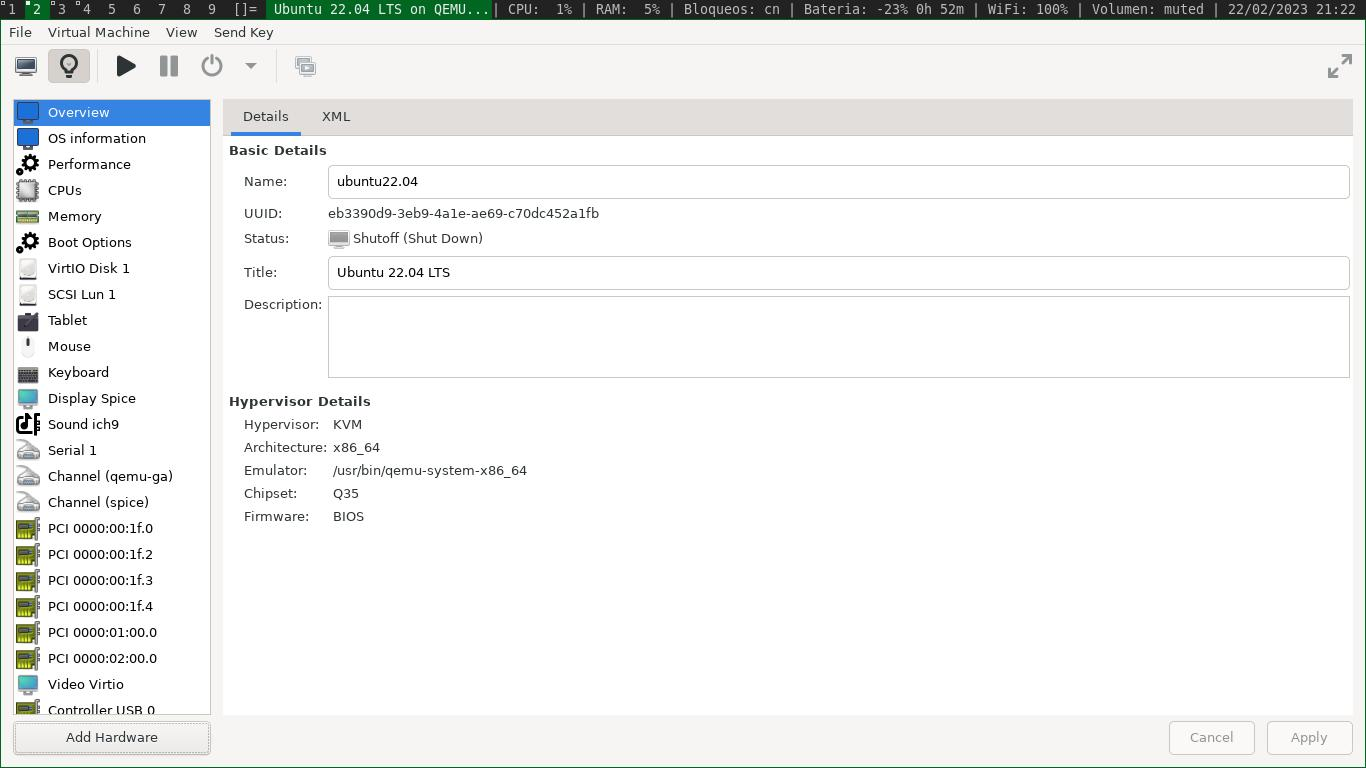
\includegraphics[width=\textwidth]{virtualMachine01}
\end{figure}
\begin{figure}[!ht]
  \caption{Información de \acrshort{so} de \acrshort{mv}}
  \centering
  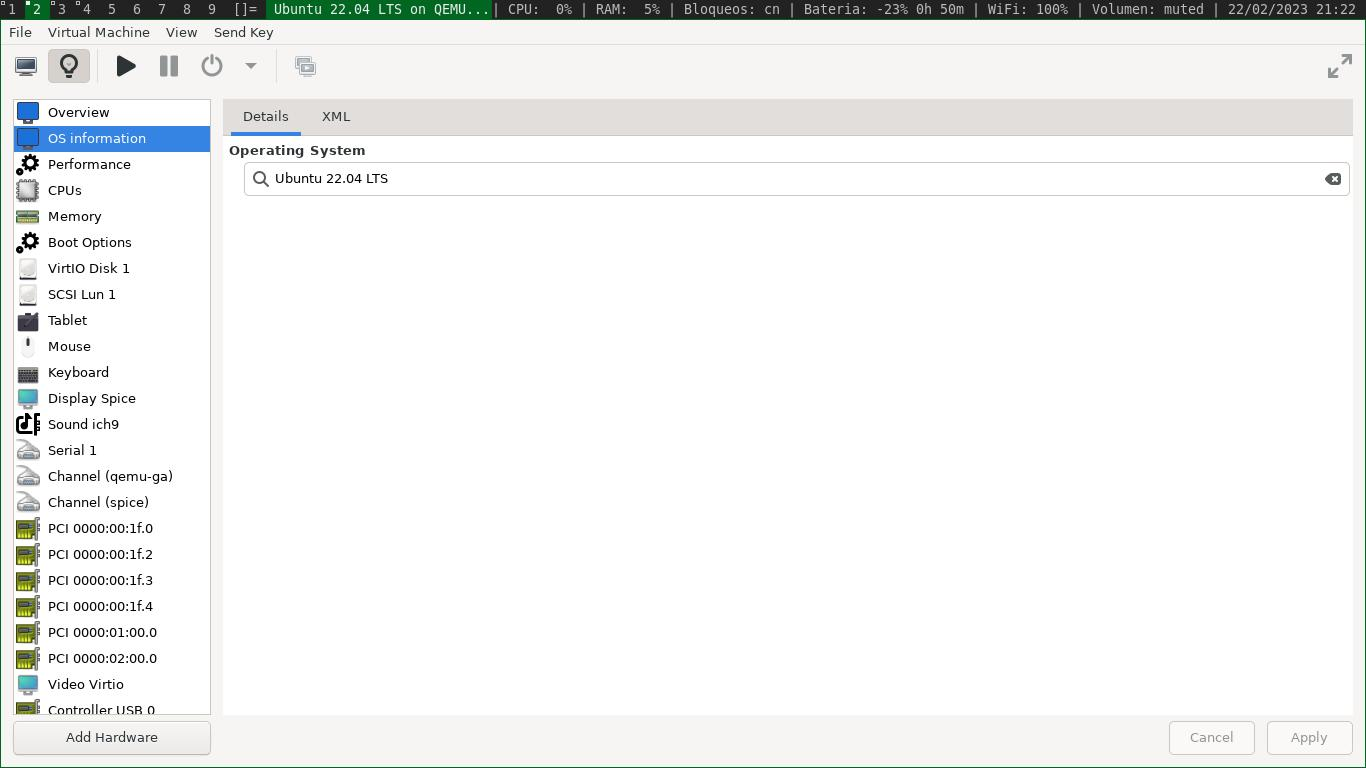
\includegraphics[width=\textwidth]{virtualMachine02}
\end{figure}
\newpage
\begin{figure}[!ht]
  \caption{\acrshort{cpu}s de \acrshort{mv}}
  \centering
  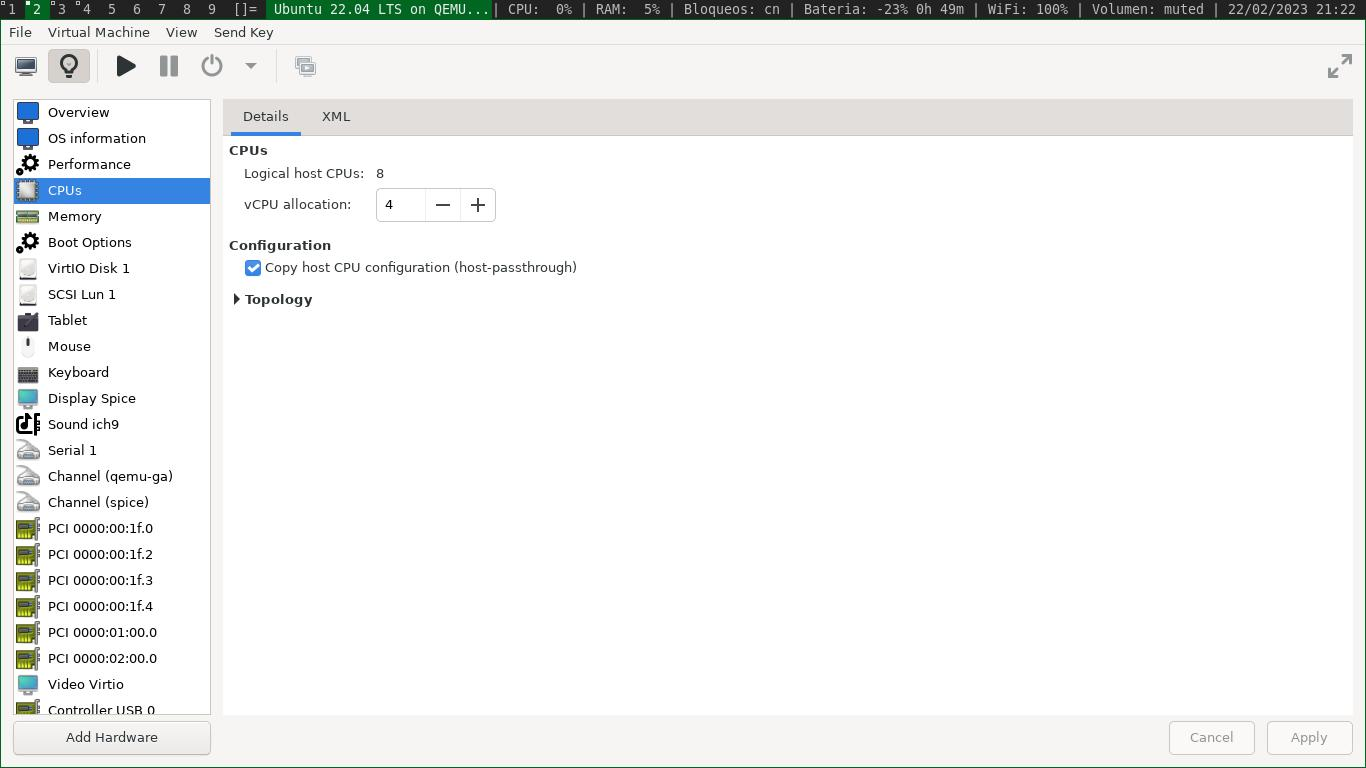
\includegraphics[width=\textwidth]{virtualMachine03}
\end{figure}
\begin{figure}[!ht]
  \caption{Memoria de \acrshort{mv}}
  \centering
  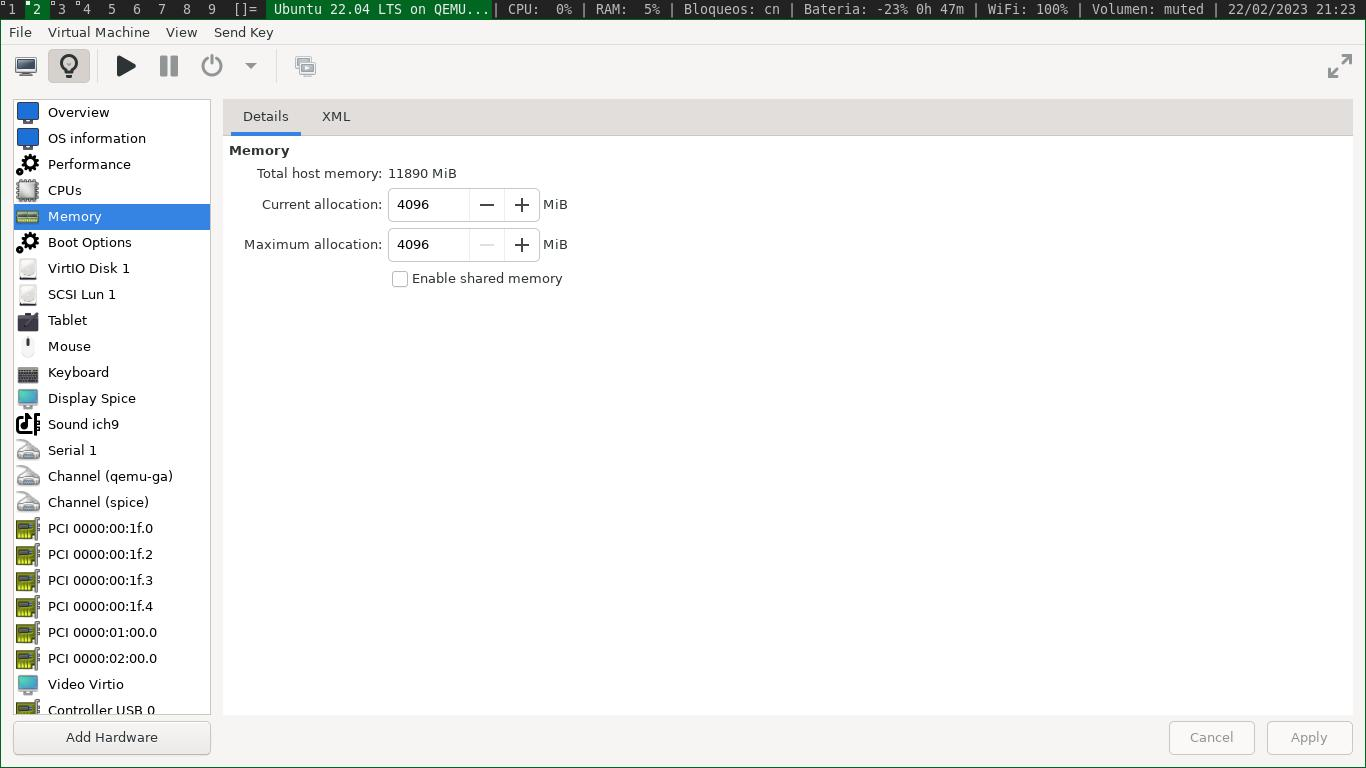
\includegraphics[width=\textwidth]{virtualMachine04}
\end{figure}
\newpage
\begin{figure}[!ht]
  \caption{Opciones de arranque de \acrshort{mv}}
  \centering
  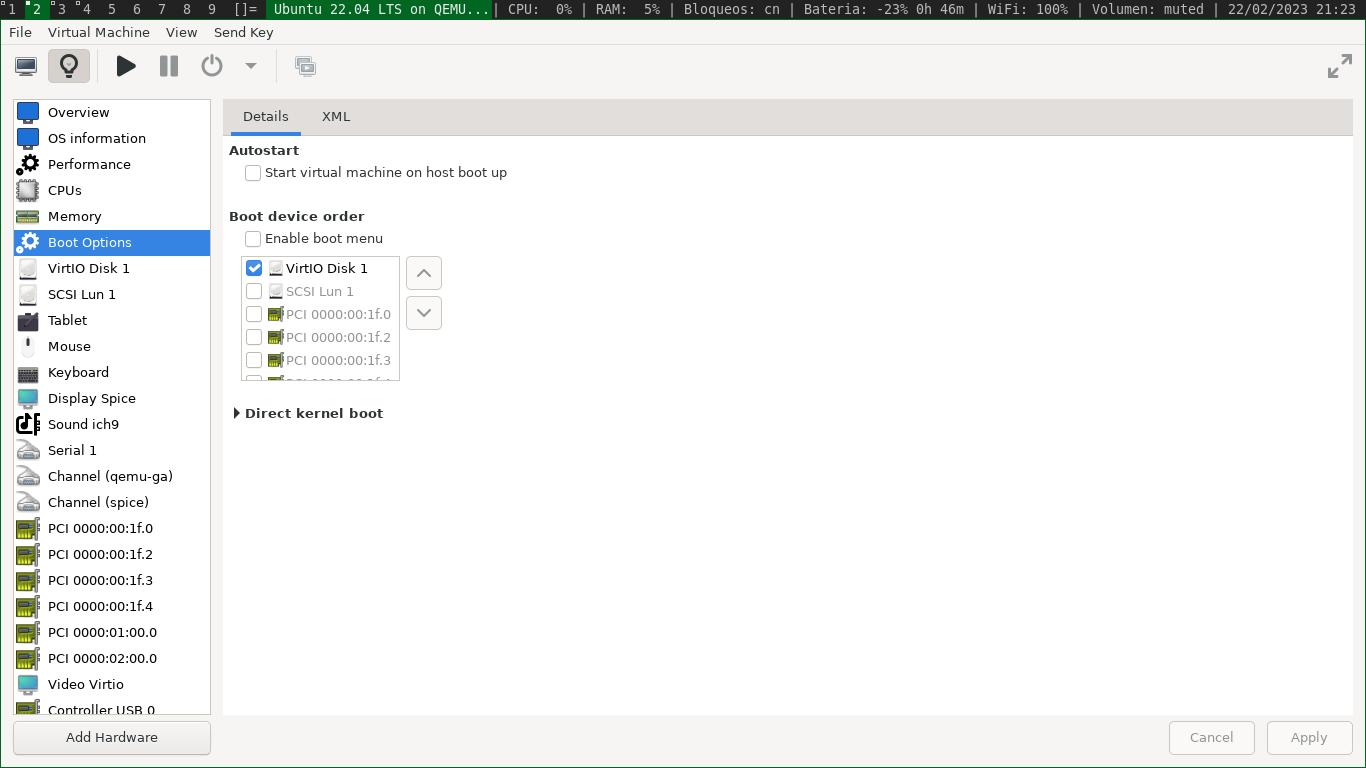
\includegraphics[width=\textwidth]{virtualMachine05}
\end{figure}
\begin{figure}[!ht]
  \caption{Disco VirtIO de \acrshort{mv}}
  \centering
  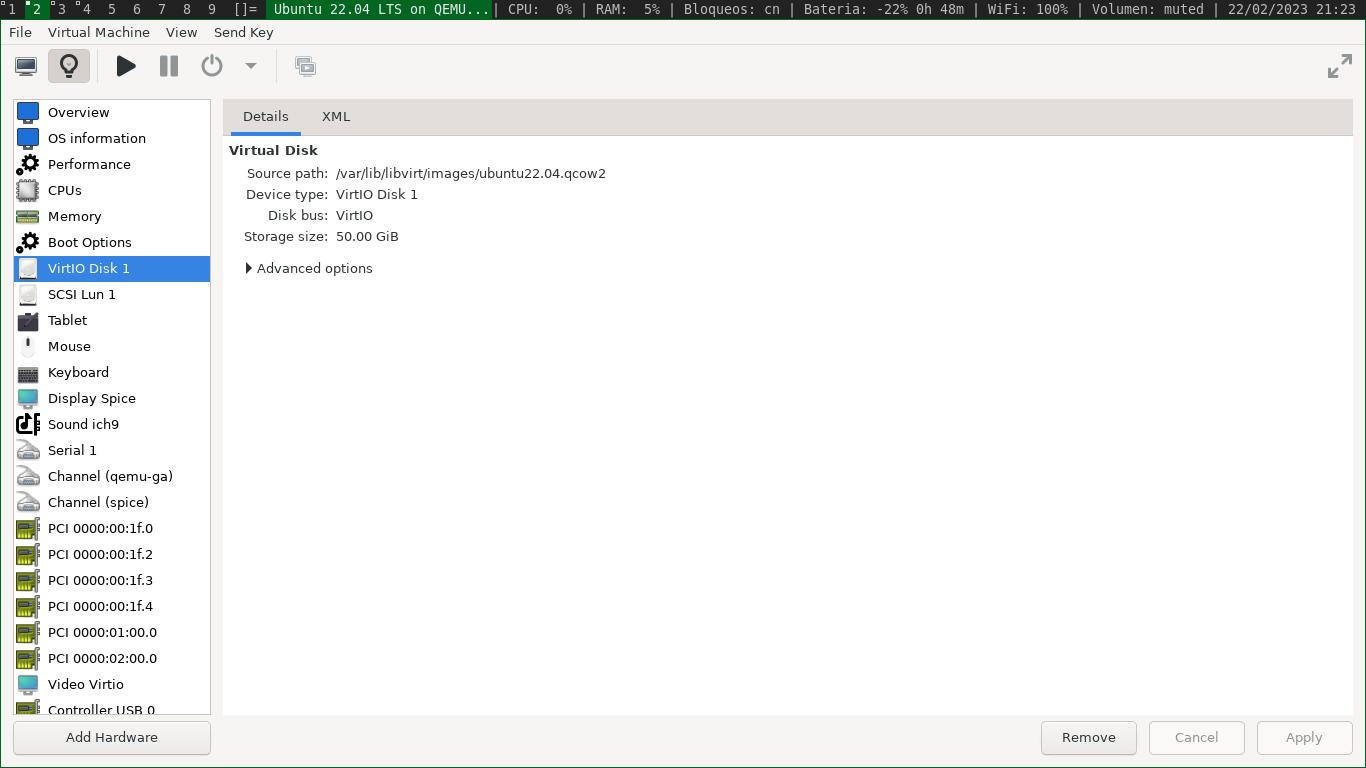
\includegraphics[width=\textwidth]{virtualMachine06}
\end{figure}
\newpage
\begin{figure}[!ht]
  \caption{Lector de discos en \acrshort{mv}}
  \centering
  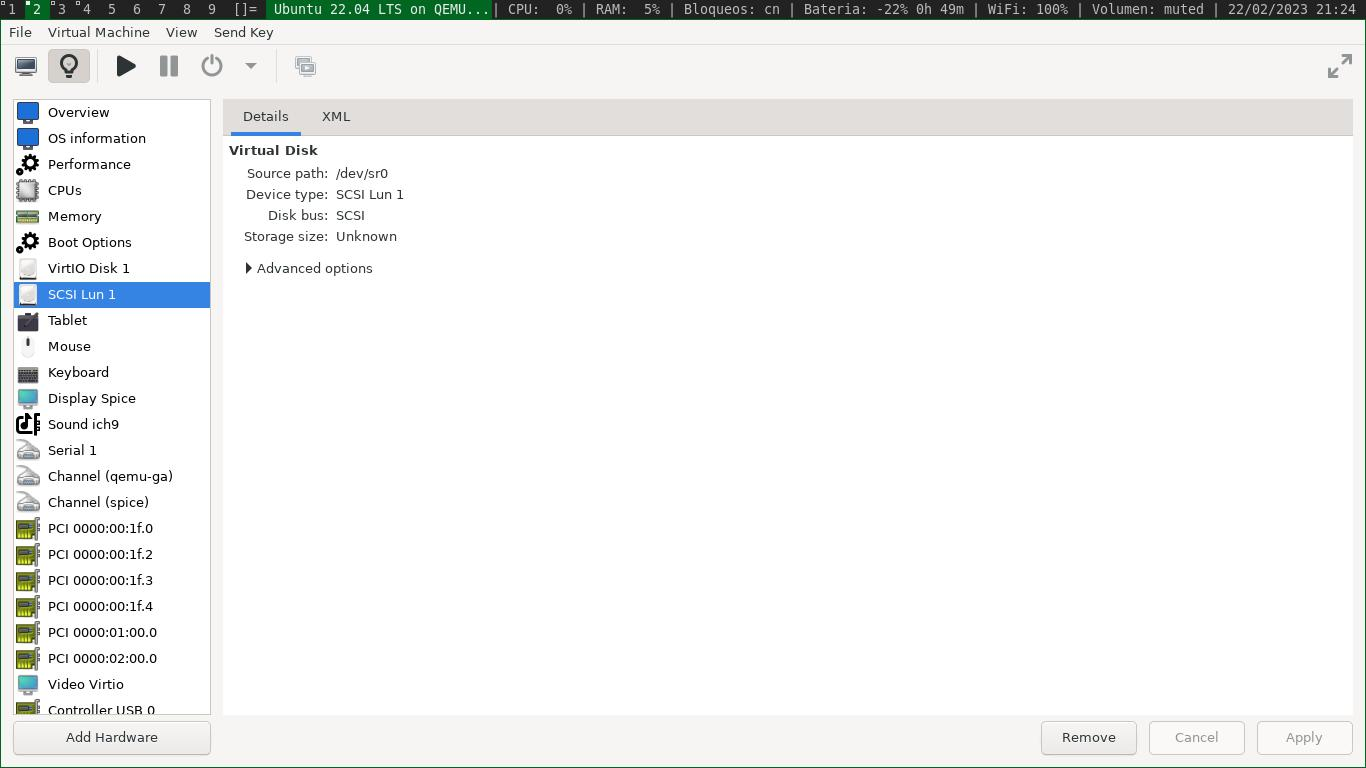
\includegraphics[width=\textwidth]{virtualMachine07}
\end{figure}
\begin{figure}[!ht]
  \caption{Tableta de \acrshort{mv}}
  \centering
  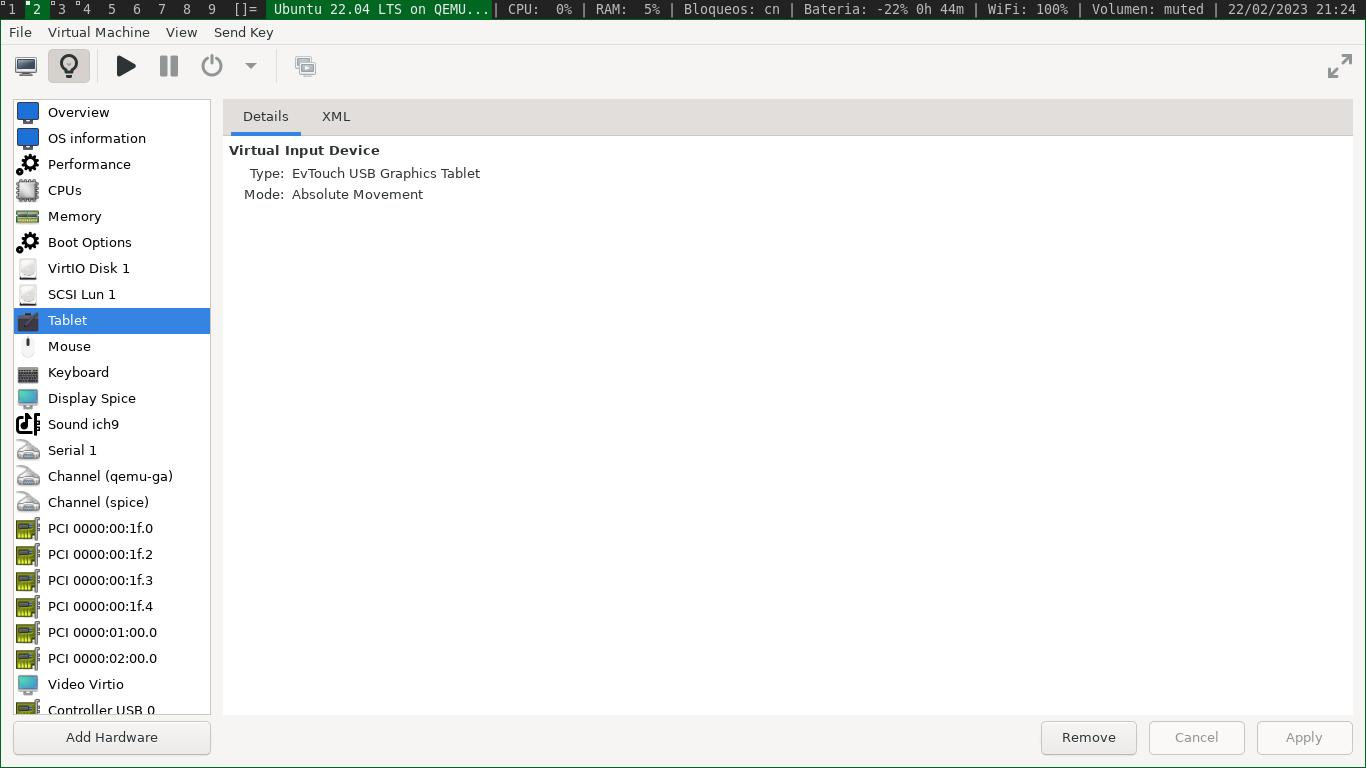
\includegraphics[width=\textwidth]{virtualMachine08}
\end{figure}
\newpage
\begin{figure}[!ht]
  \caption{Ratón de \acrshort{mv}}
  \centering
  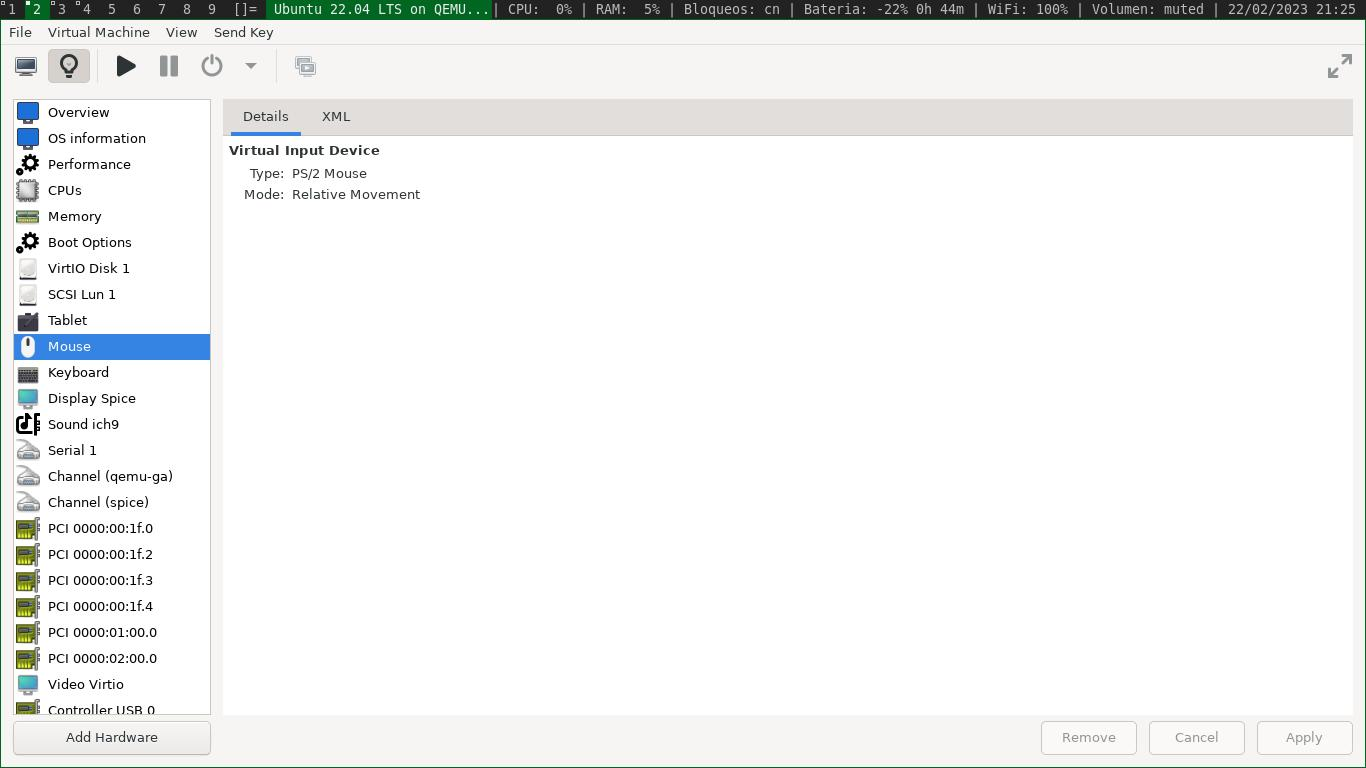
\includegraphics[width=\textwidth]{virtualMachine09}
\end{figure}
\begin{figure}[!ht]
  \caption{Teclado de \acrshort{mv}}
  \centering
  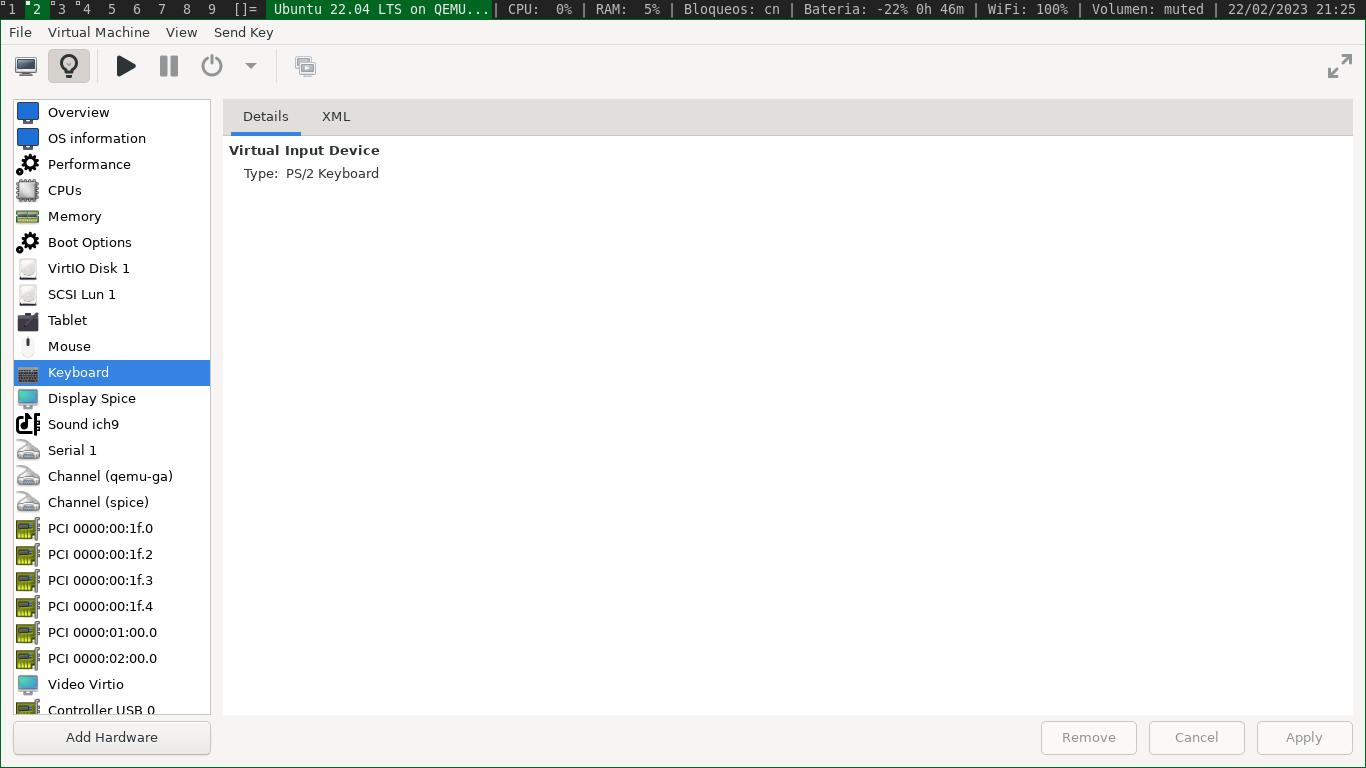
\includegraphics[width=\textwidth]{virtualMachine10}
\end{figure}
\newpage
\begin{figure}[!ht]
  \caption{Servidor de pantalla de \acrshort{mv}}
  \centering
  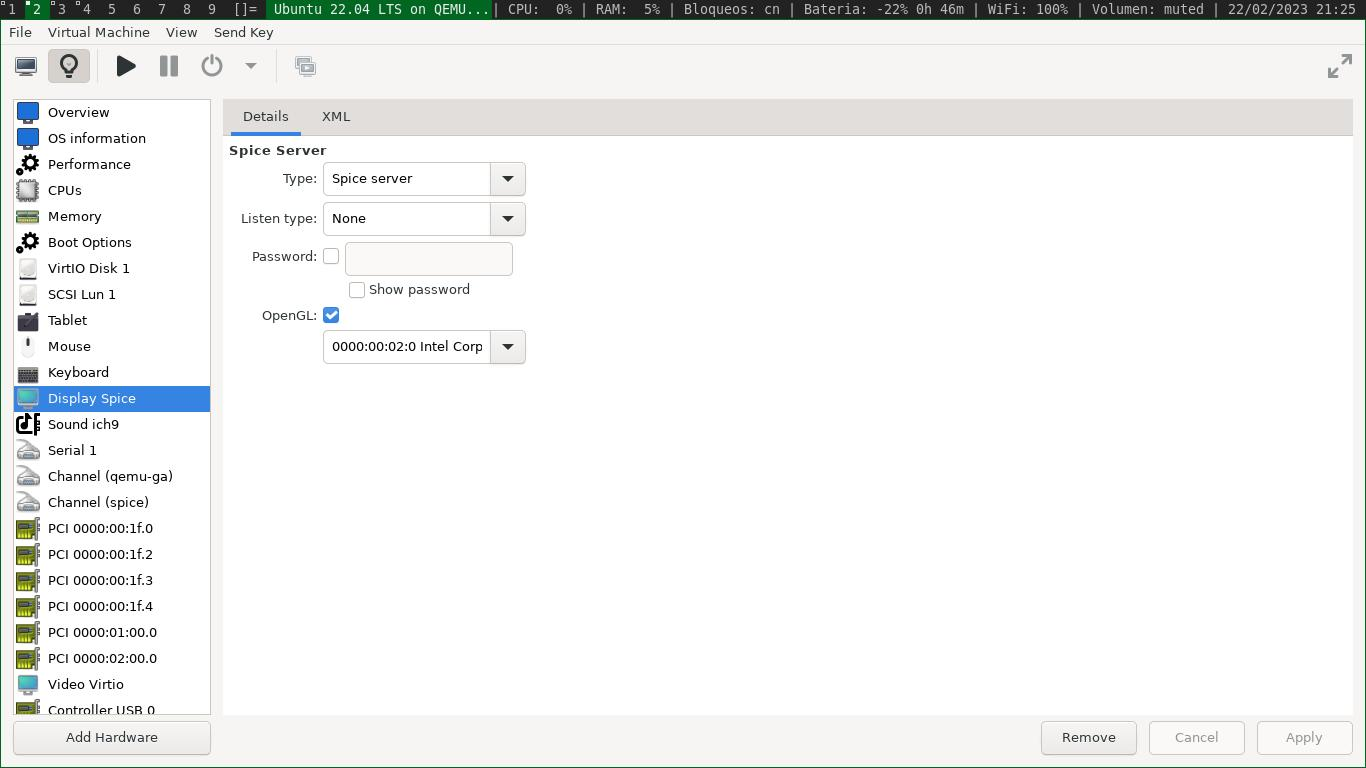
\includegraphics[width=\textwidth]{virtualMachine11}
\end{figure}
\begin{figure}[!ht]
  \caption{Sonido de \acrshort{mv}}
  \centering
  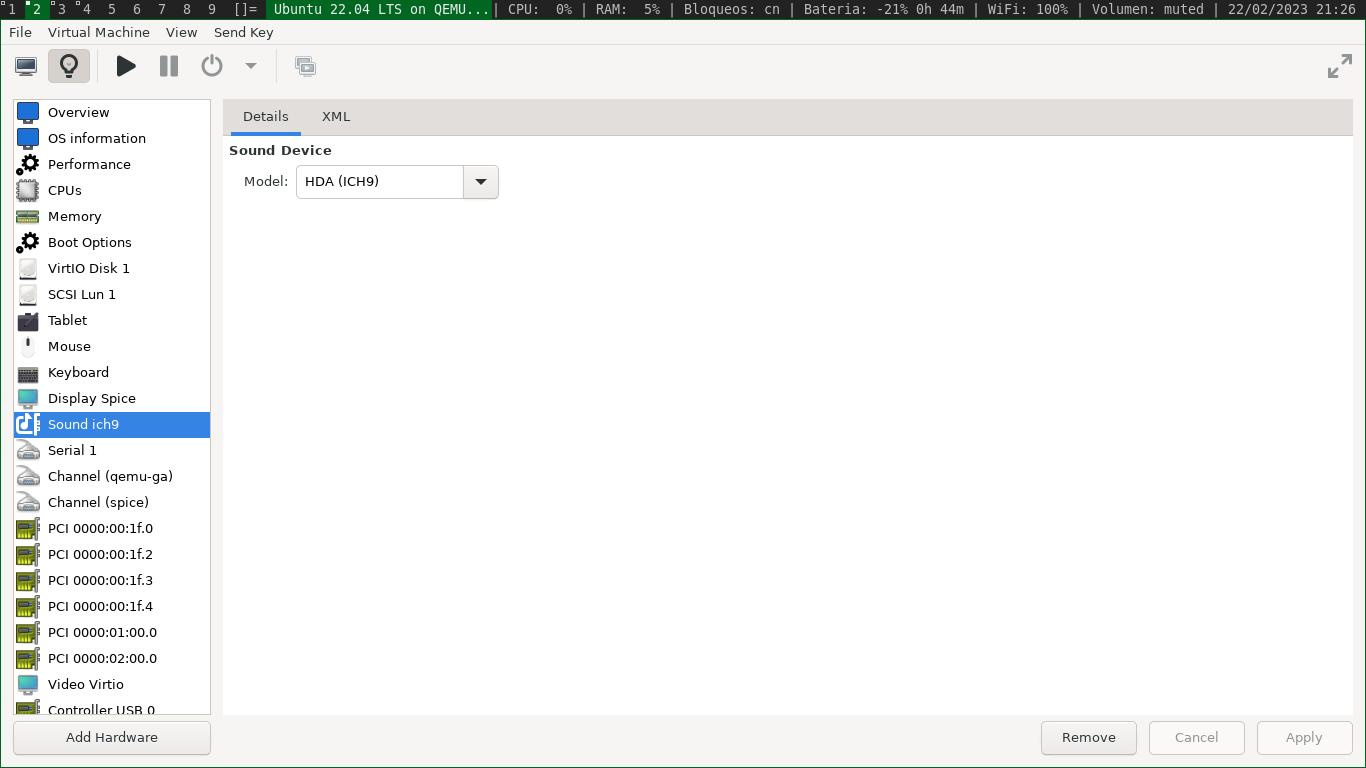
\includegraphics[width=\textwidth]{virtualMachine12}
\end{figure}
\newpage
\begin{figure}[!ht]
  \caption{Dispositivo Serial 1 de \acrshort{mv}}
  \centering
  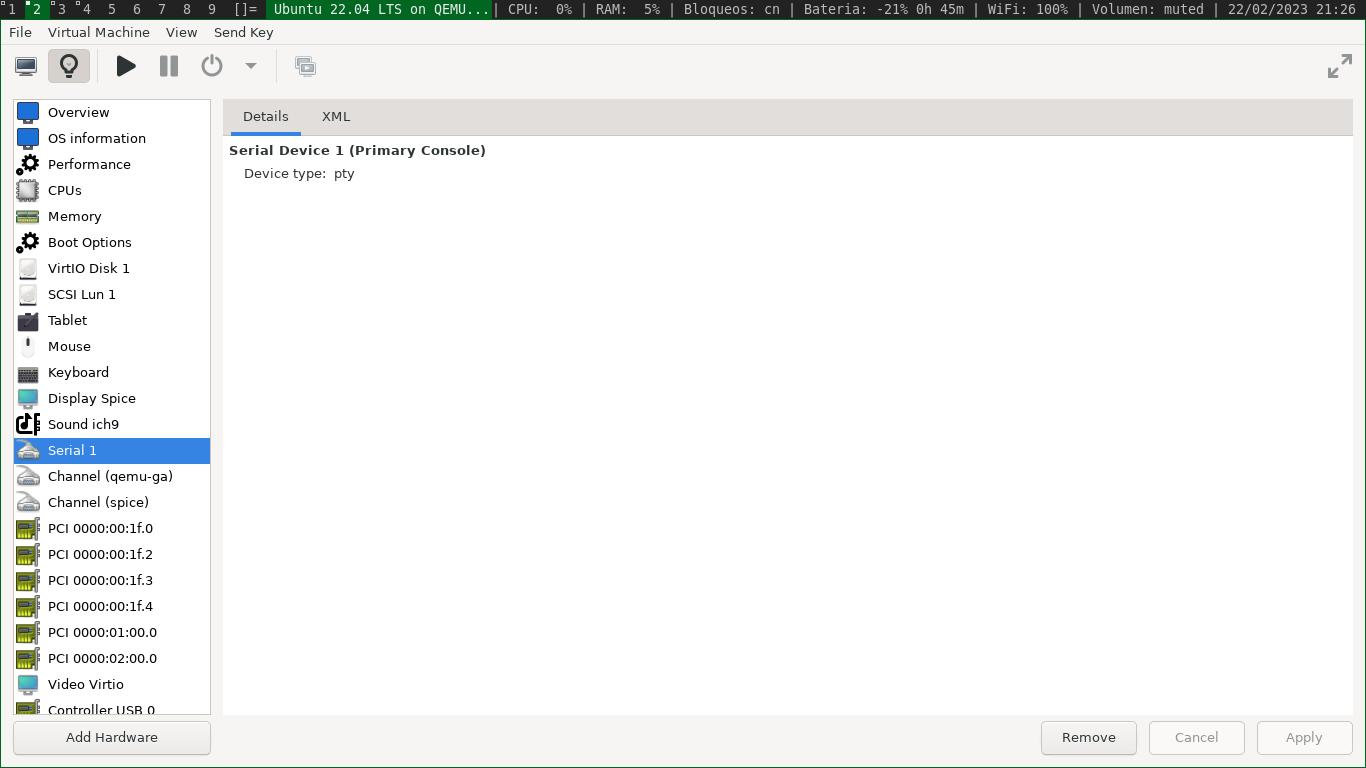
\includegraphics[width=\textwidth]{virtualMachine13}
\end{figure}
\begin{figure}[!ht]
  \caption{Canal qemu-ga de \acrshort{mv}}
  \centering
  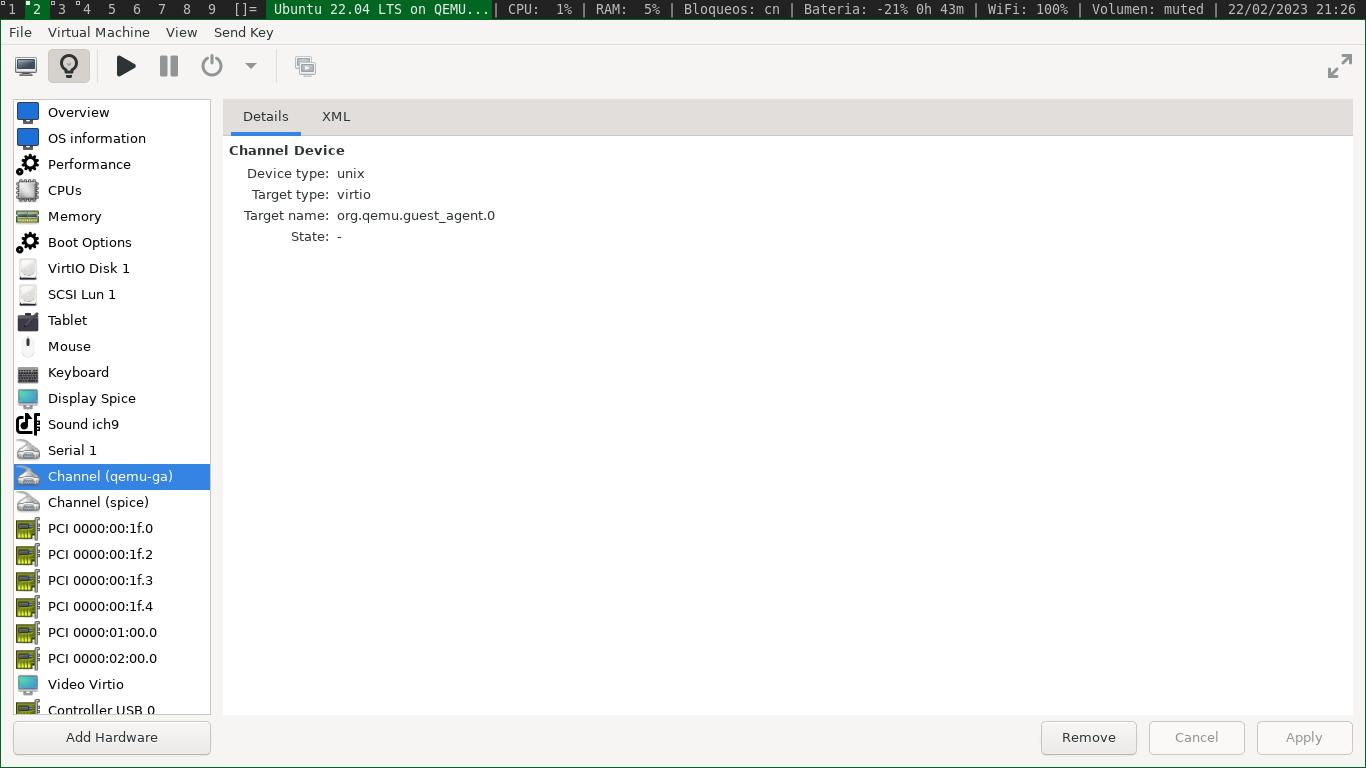
\includegraphics[width=\textwidth]{virtualMachine14}
\end{figure}
\newpage
\begin{figure}[!ht]
  \caption{Canal spice de \acrshort{mv}}
  \centering
  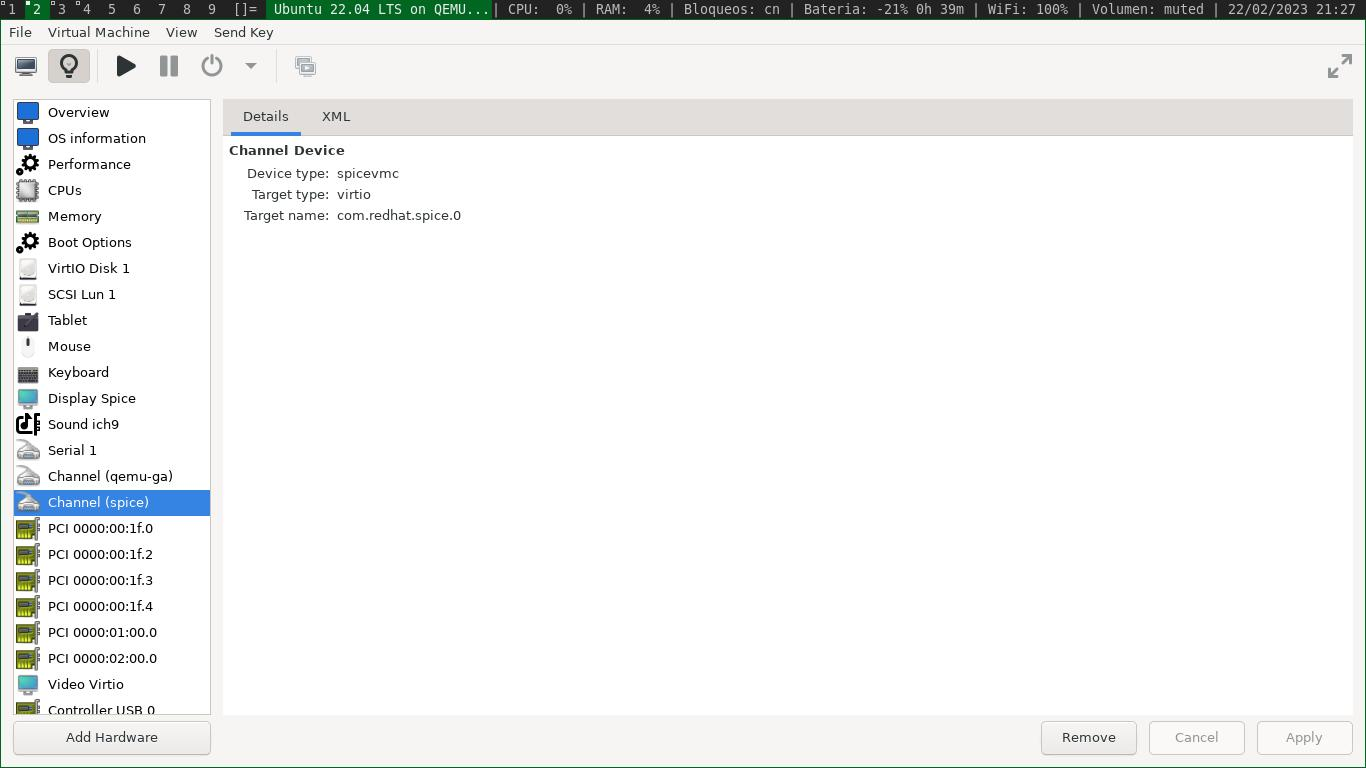
\includegraphics[width=\textwidth]{virtualMachine15}
\end{figure}
\begin{figure}[!ht]
  \caption{Controlador eSPI en \acrshort{mv}}
  \centering
  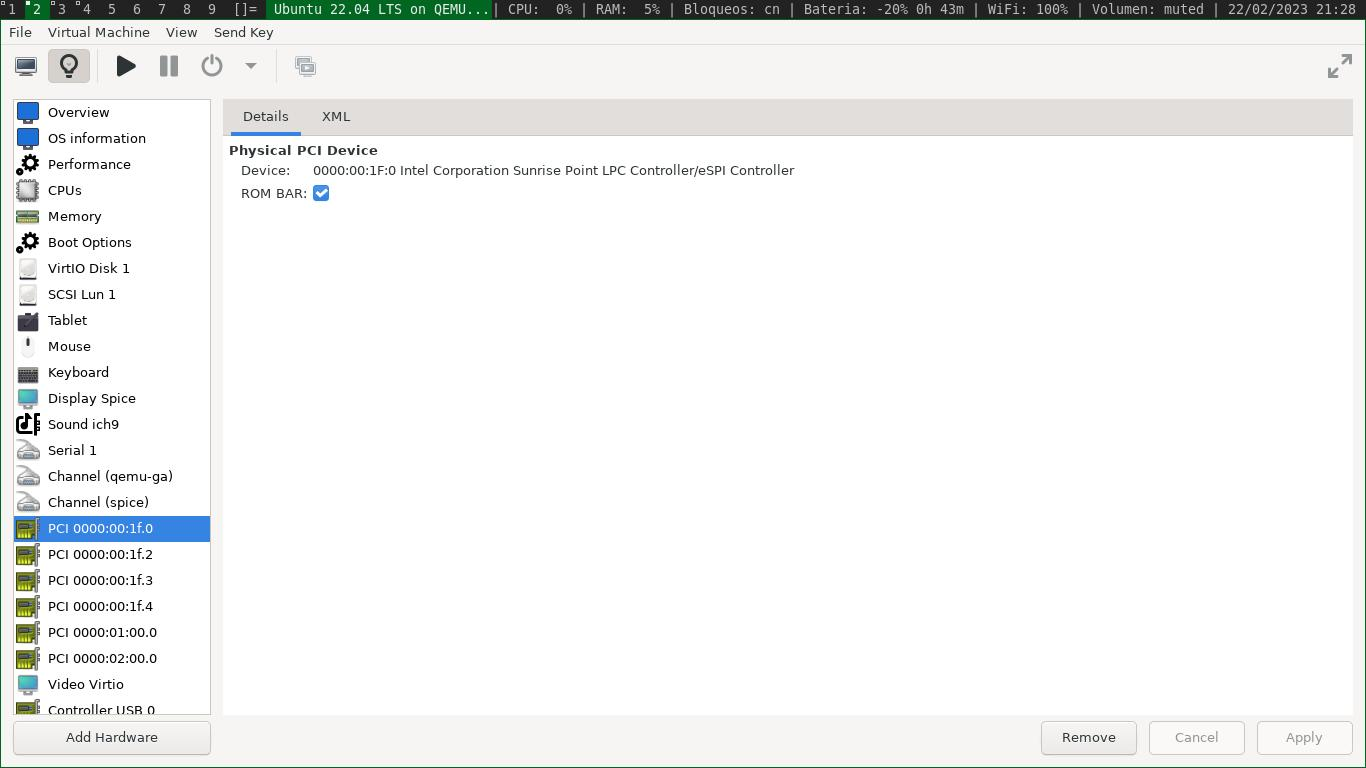
\includegraphics[width=\textwidth]{virtualMachine16}
\end{figure}
\newpage
\begin{figure}[!ht]
  \caption{Controlador de gestión de energía en \acrshort{mv}}
  \centering
  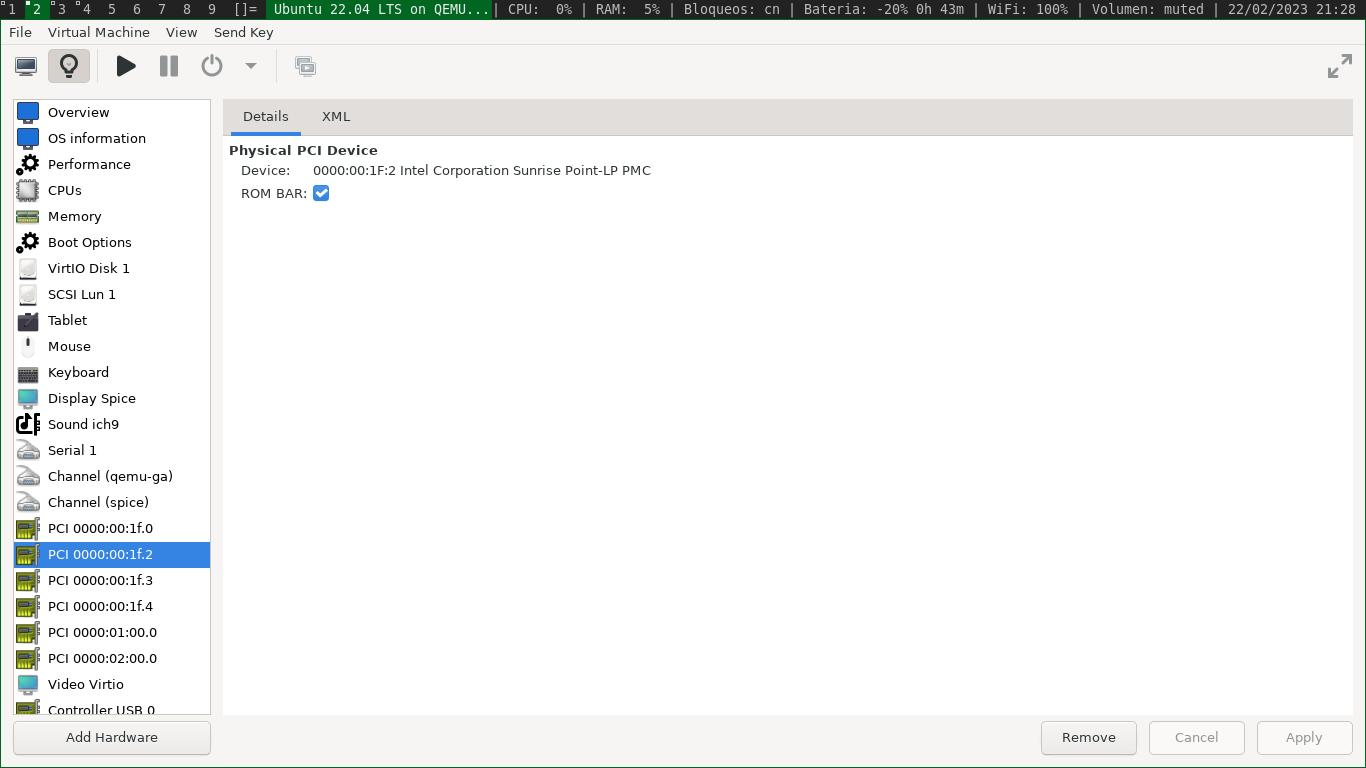
\includegraphics[width=\textwidth]{virtualMachine17}
\end{figure}
\begin{figure}[!ht]
  \caption{Controlador de Audio HD en \acrshort{mv}}
  \centering
  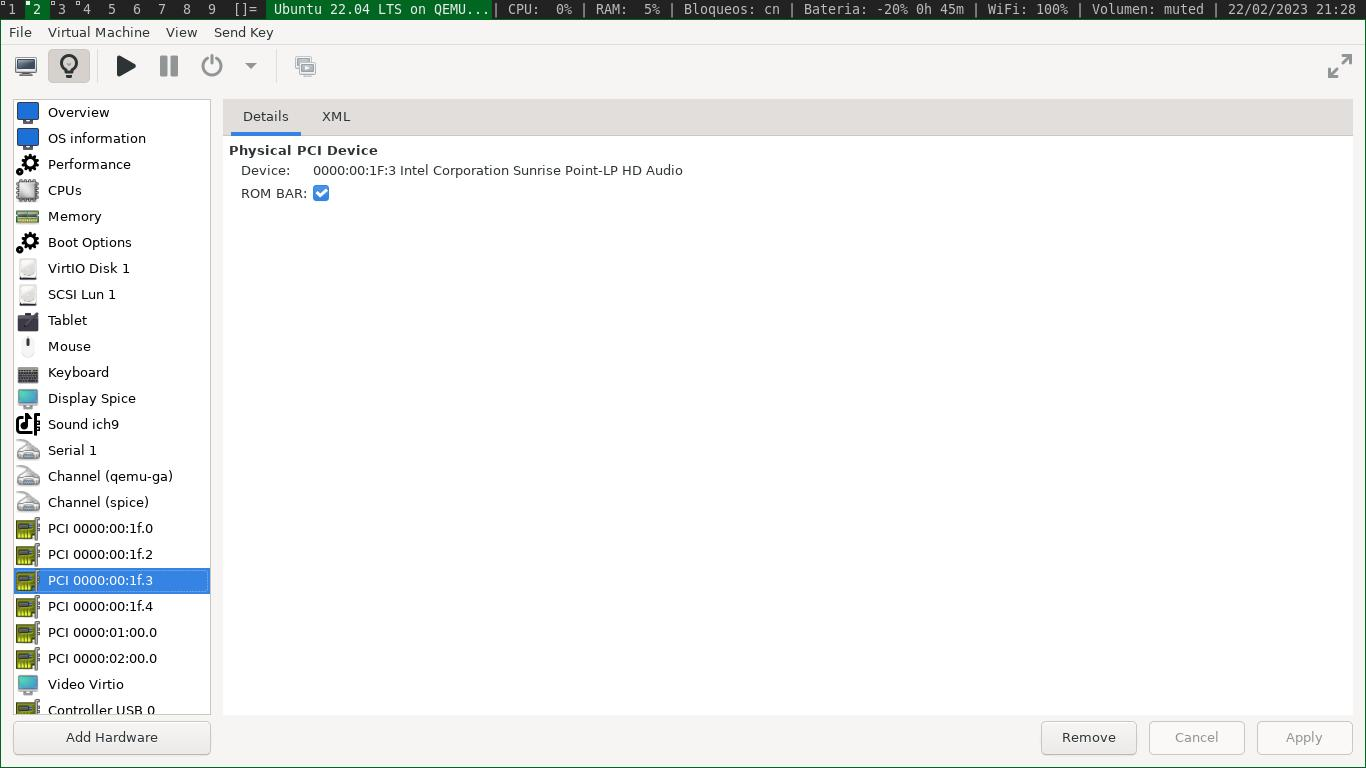
\includegraphics[width=\textwidth]{virtualMachine18}
\end{figure}
\newpage
\begin{figure}[!ht]
  \caption{Bus de gestión del sistema en \acrshort{mv}}
  \centering
  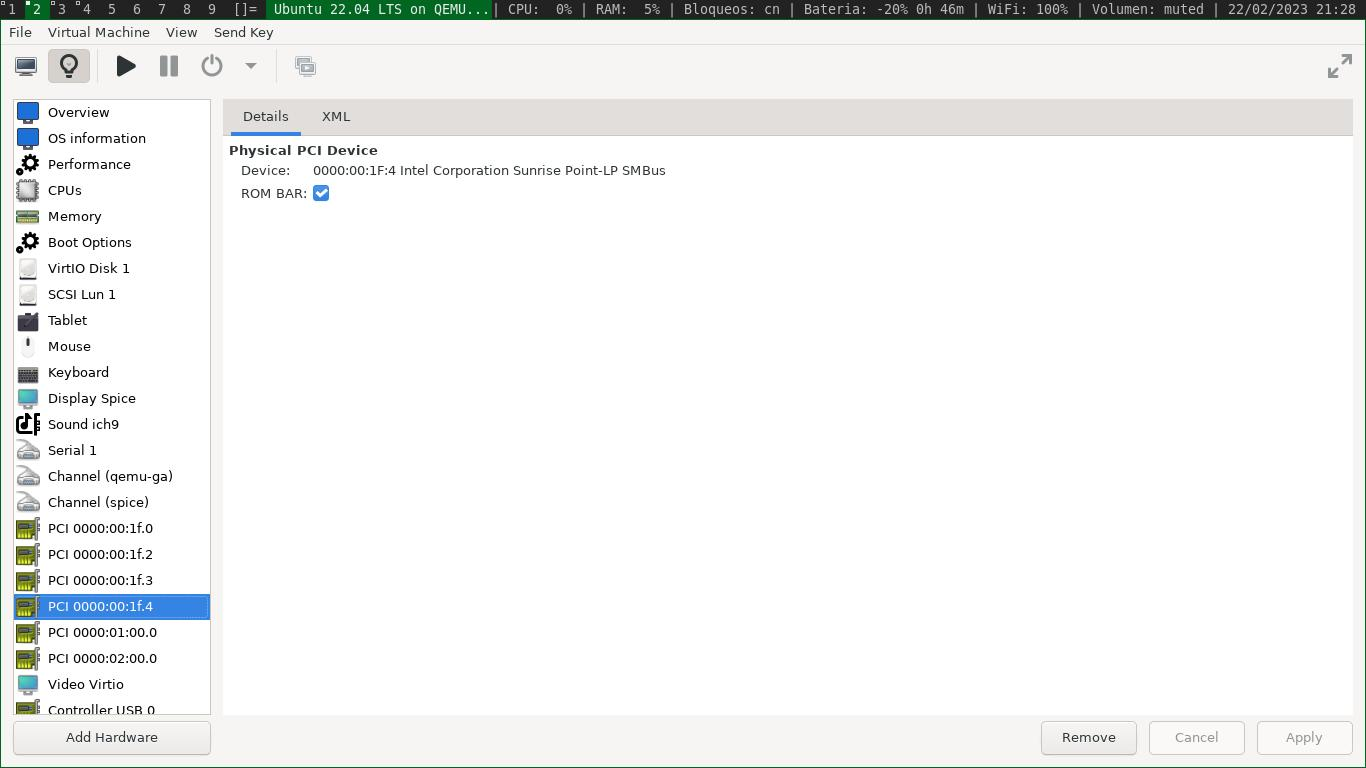
\includegraphics[width=\textwidth]{virtualMachine19}
\end{figure}
\begin{figure}[!ht]
  \caption{Controlador de Ethernet en \acrshort{mv}}
  \centering
  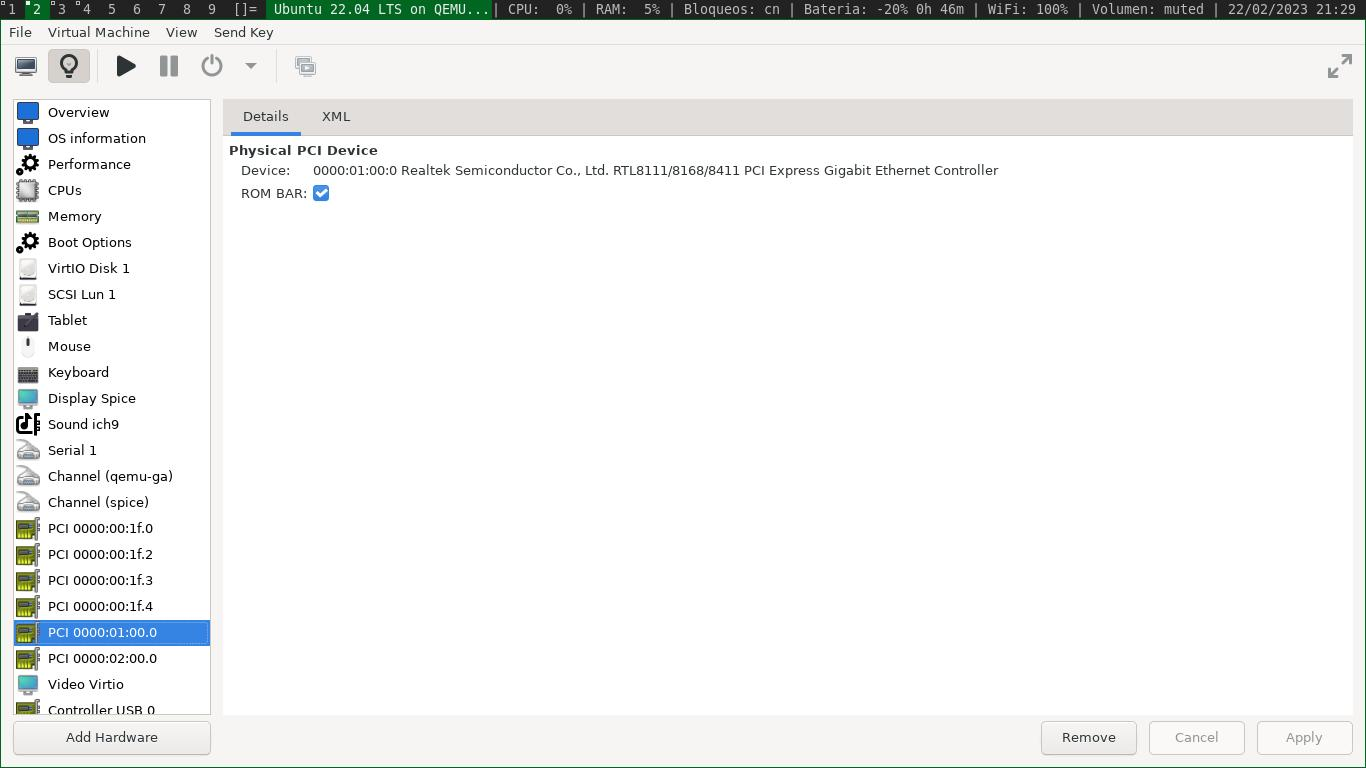
\includegraphics[width=\textwidth]{virtualMachine20}
\end{figure}
\newpage
\begin{figure}[!ht]
  \caption{Controlador de WiFi en \acrshort{mv}}
  \centering
  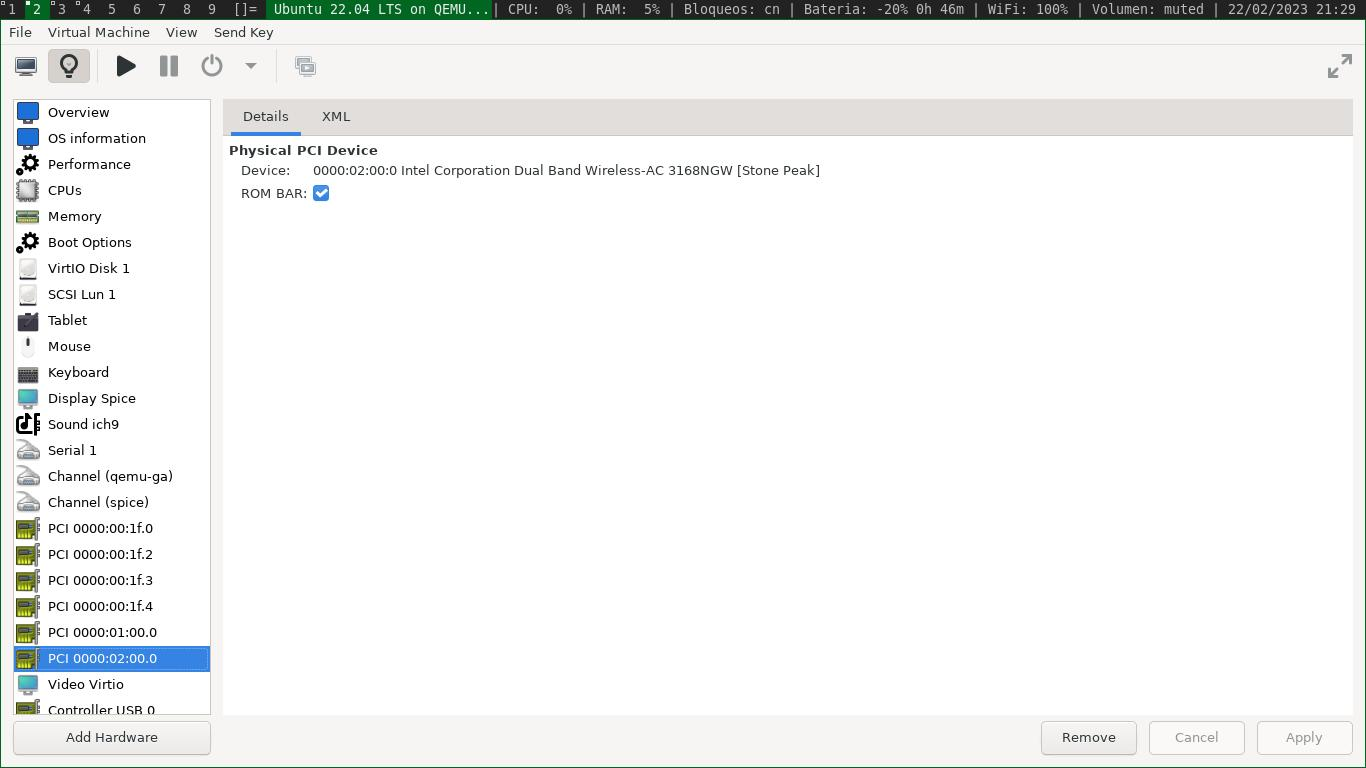
\includegraphics[width=\textwidth]{virtualMachine21}
\end{figure}
\begin{figure}[!ht]
  \caption{Modelo de video de \acrshort{mv}}
  \centering
  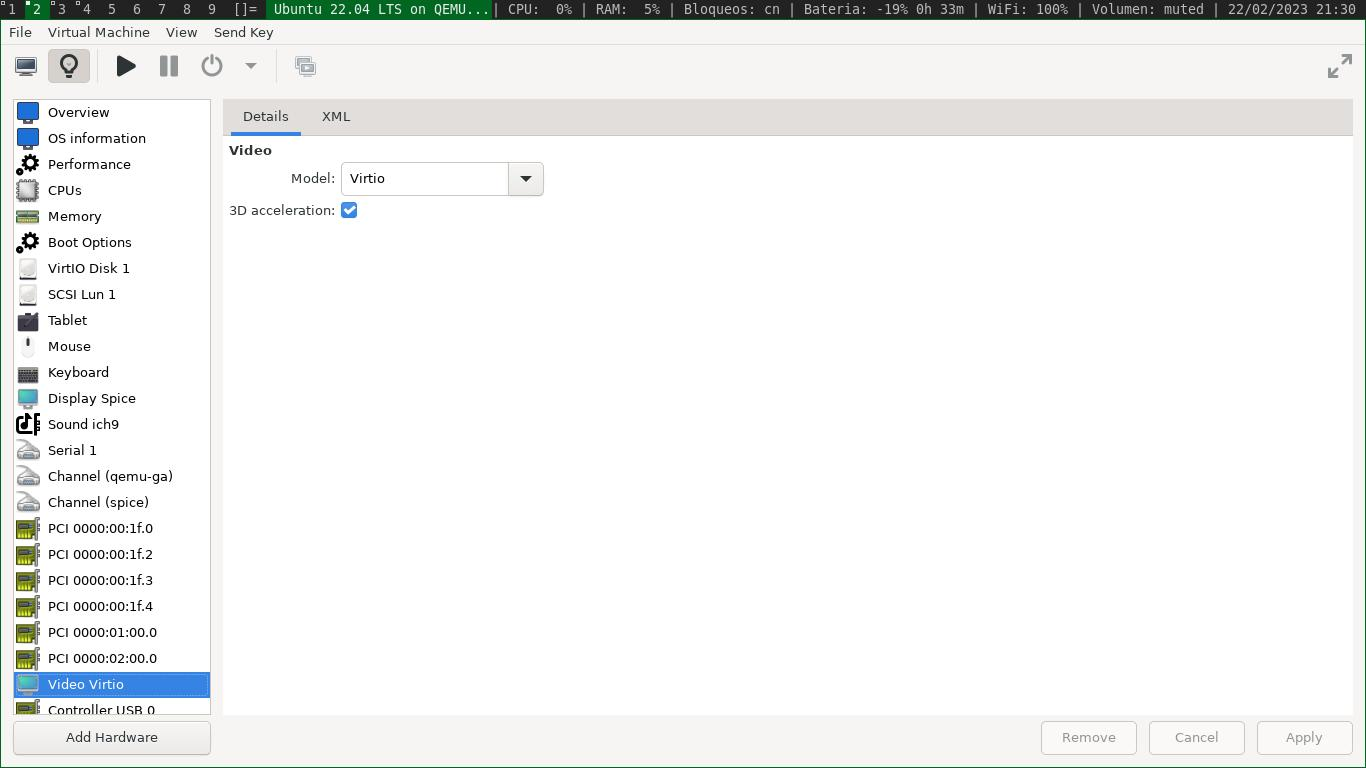
\includegraphics[width=\textwidth]{virtualMachine22}
\end{figure}
\newpage
\begin{figure}[!ht]
  \caption{Controlador USB de \acrshort{mv}}
  \centering
  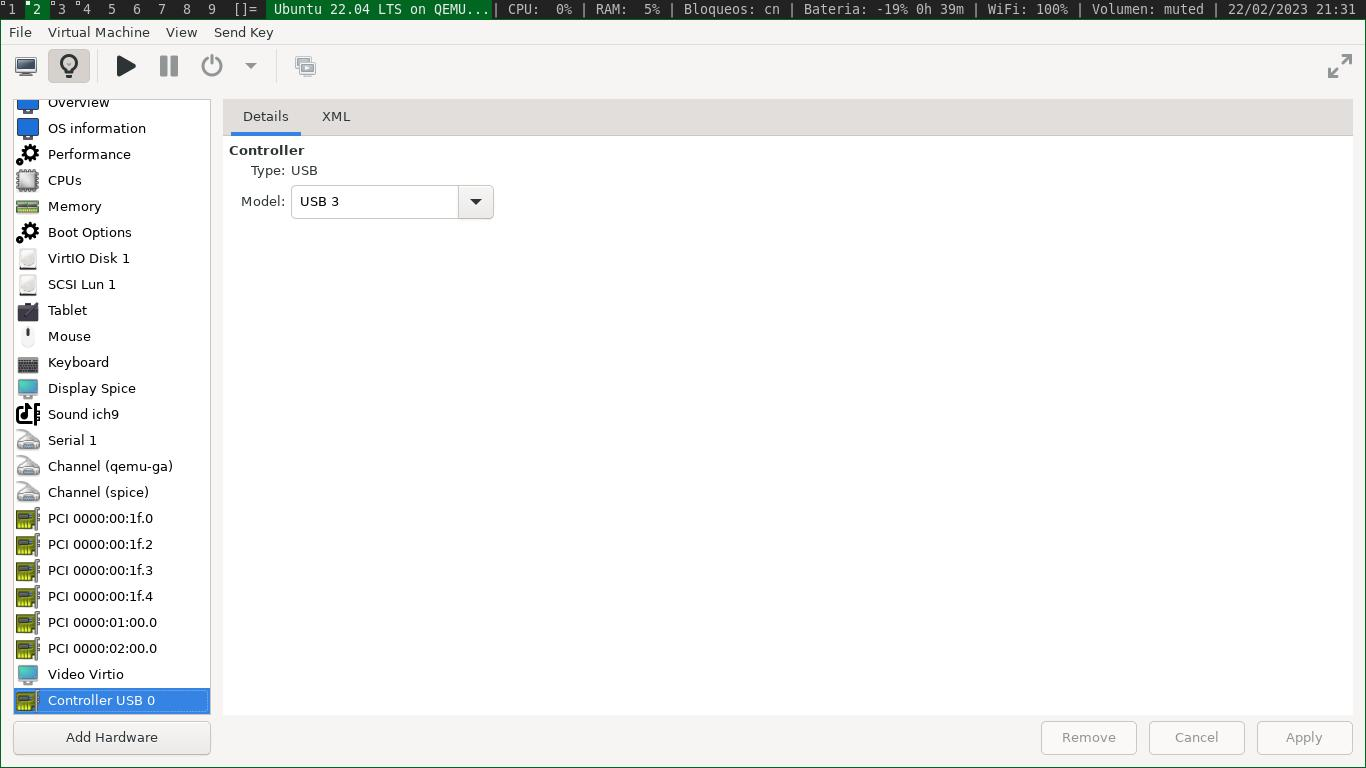
\includegraphics[width=\textwidth]{virtualMachine23}
\end{figure}
\begin{figure}[!ht]
  \caption{Controlador PCIe de \acrshort{mv}}
  \centering
  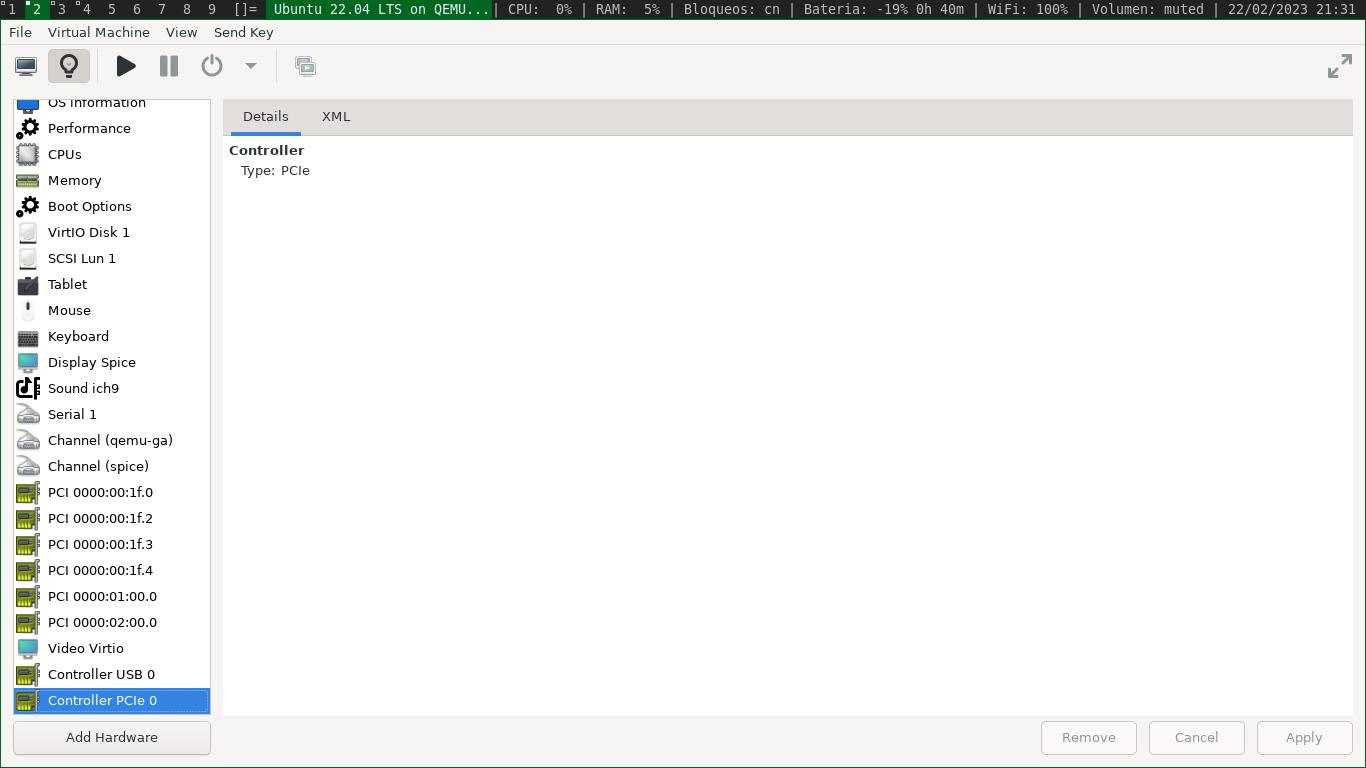
\includegraphics[width=\textwidth]{virtualMachine24}
\end{figure}
\newpage
\begin{figure}[!ht]
  \caption{Controlador PCI de \acrshort{mv}}
  \centering
  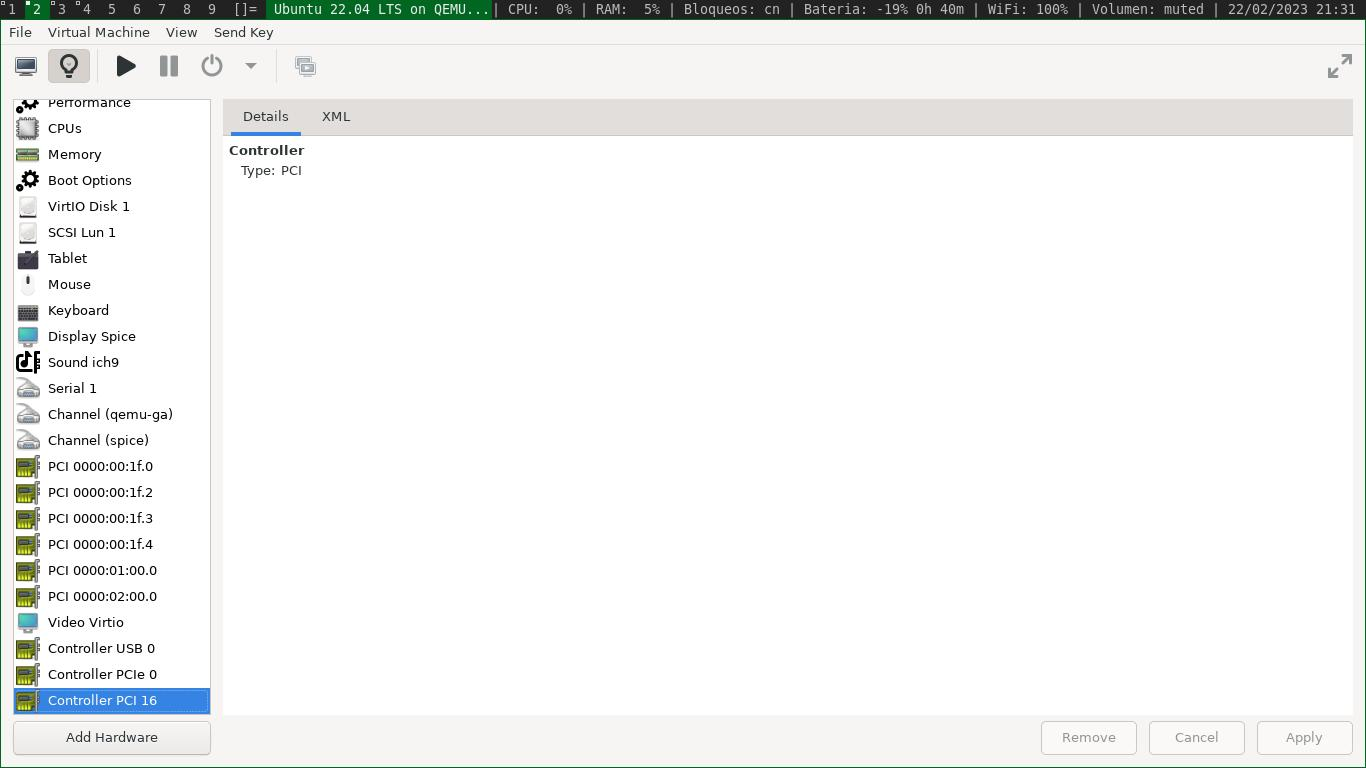
\includegraphics[width=\textwidth]{virtualMachine25}
\end{figure}
\begin{figure}[!ht]
  \caption{Controlador SATA de \acrshort{mv}}
  \centering
  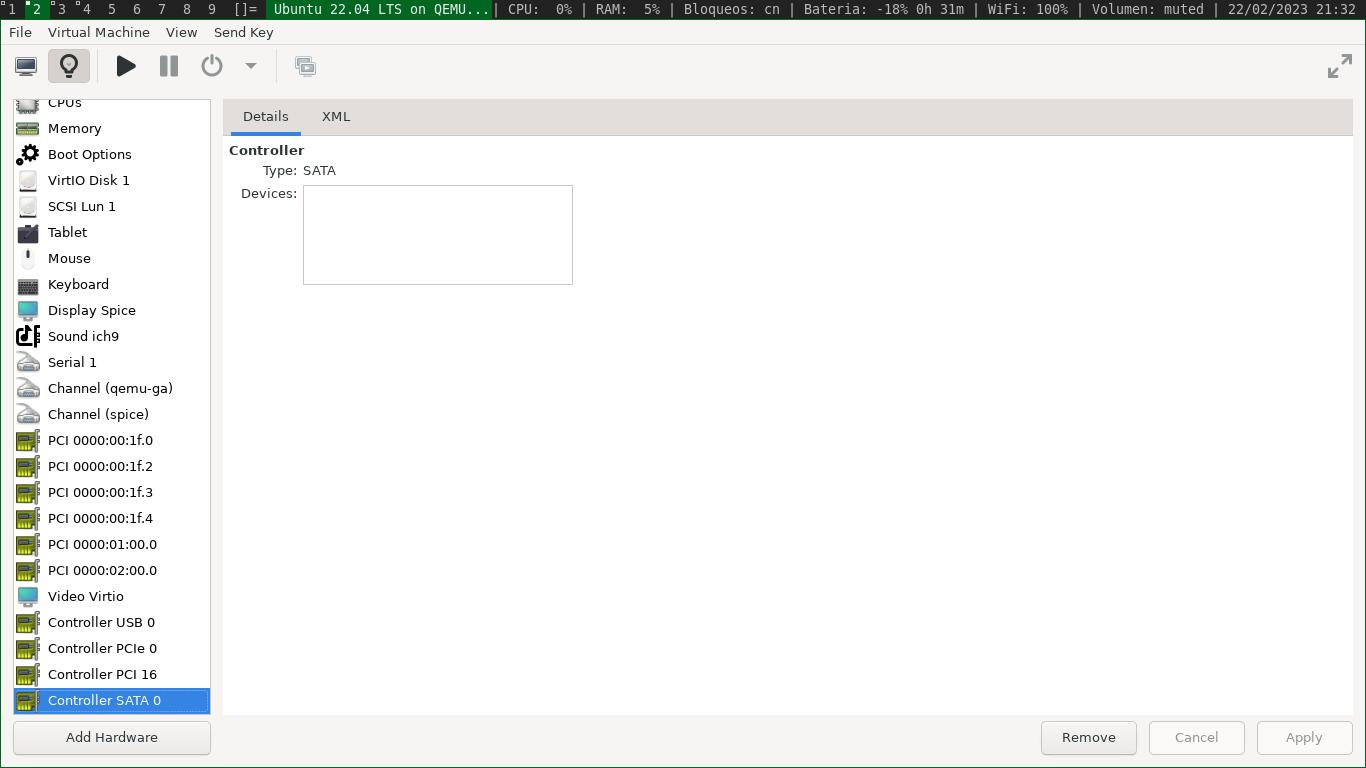
\includegraphics[width=\textwidth]{virtualMachine26}
\end{figure}
\newpage
\begin{figure}[!ht]
  \caption{Controlador Serial de \acrshort{mv}}
  \centering
  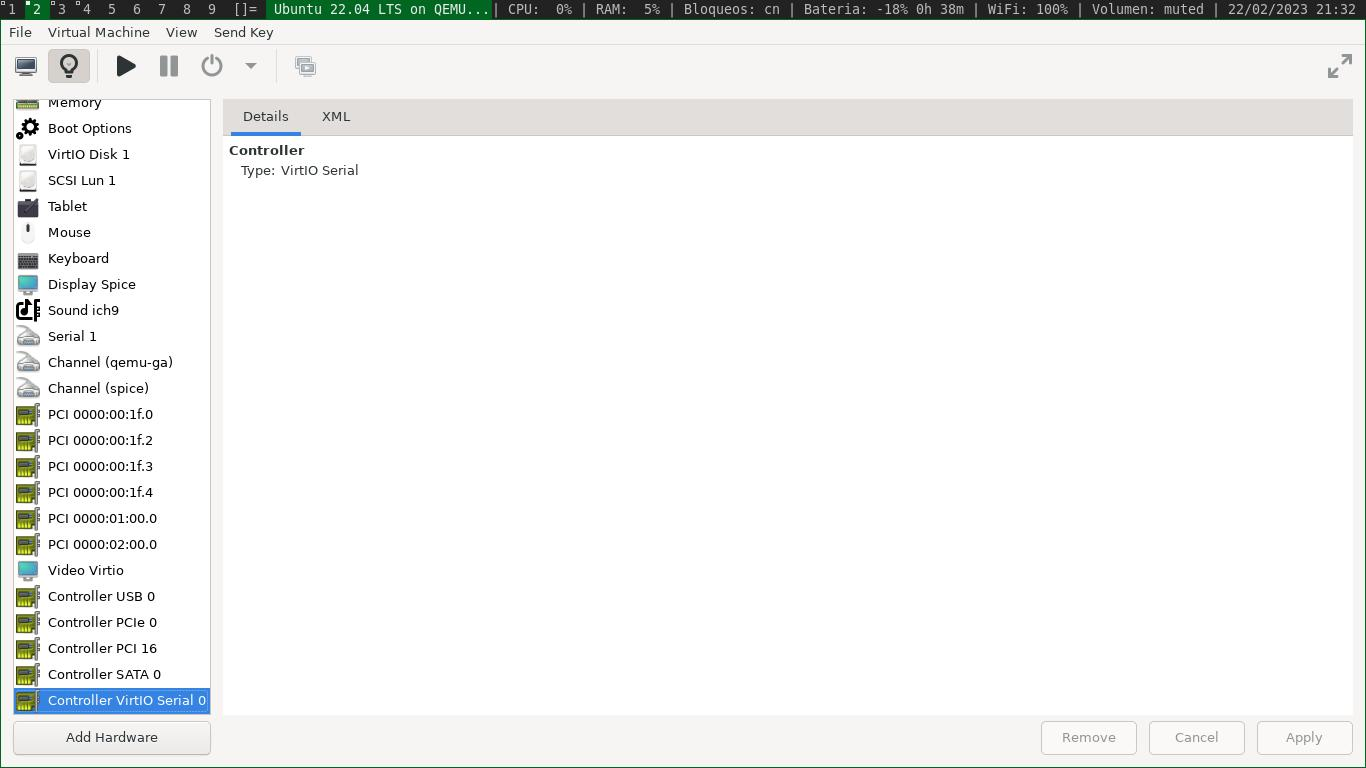
\includegraphics[width=\textwidth]{virtualMachine27}
\end{figure}
\begin{figure}[!ht]
  \caption{Controlador de lector de disco de \acrshort{mv}}
  \centering
  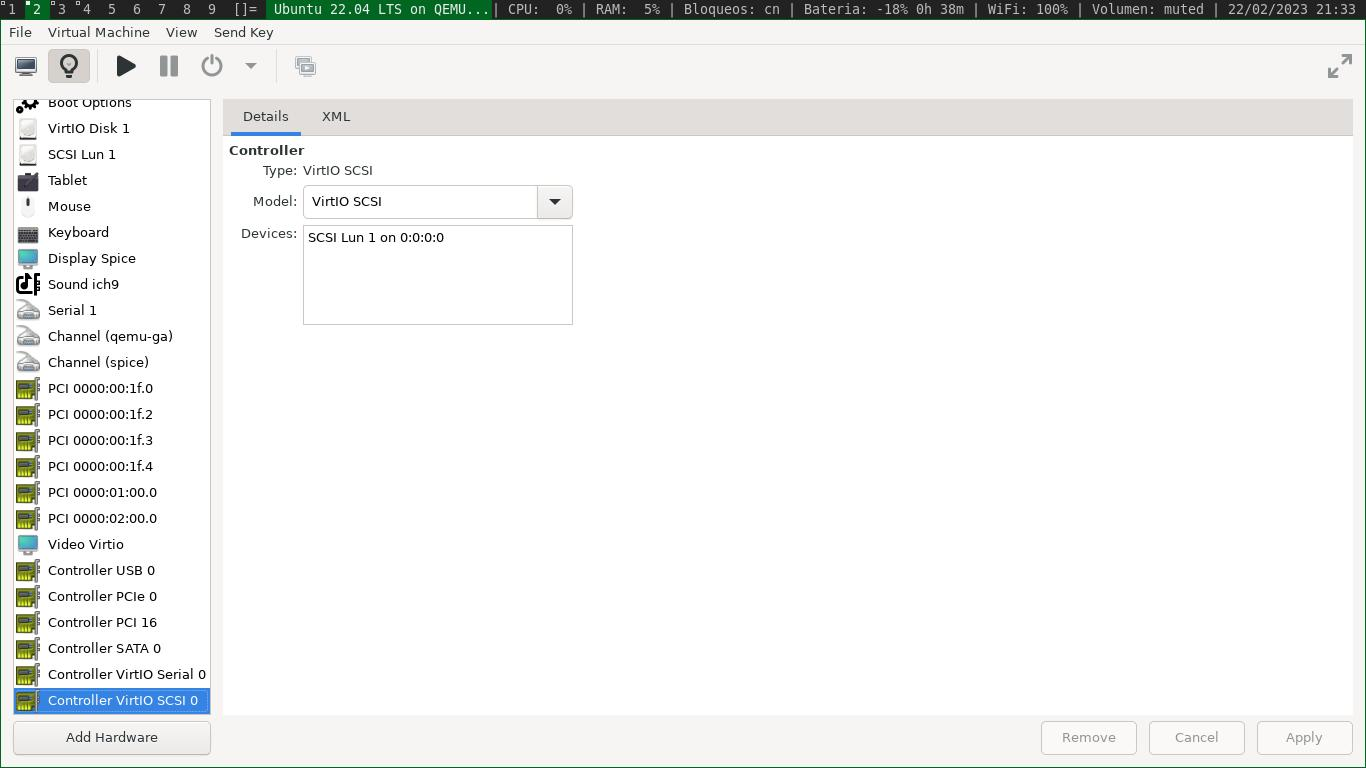
\includegraphics[width=\textwidth]{virtualMachine28}
\end{figure}
\newpage
\begin{figure}[!ht]
  \caption{Redoreccionador USB 1 de \acrshort{mv}}
  \centering
  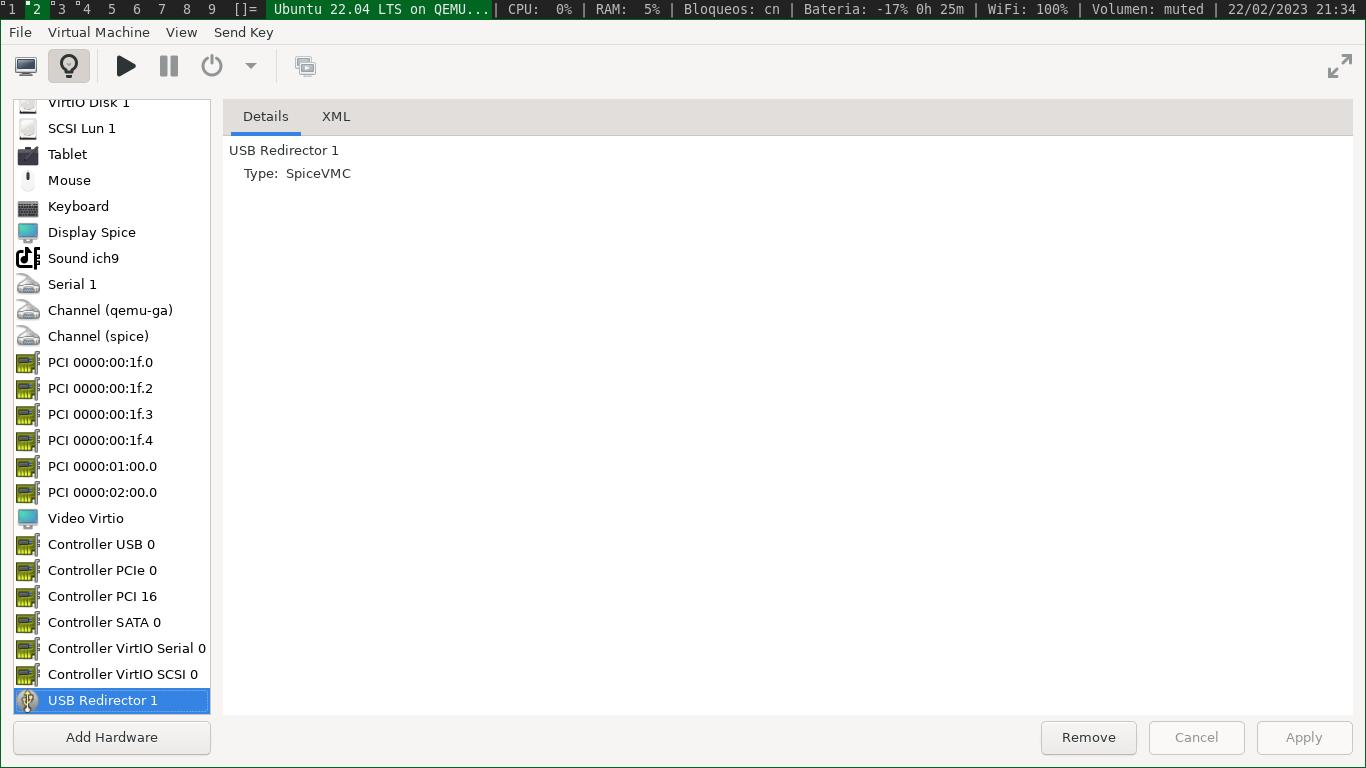
\includegraphics[width=\textwidth]{virtualMachine29}
\end{figure}
\begin{figure}[!ht]
  \caption{Redoreccionador USB 2 de \acrshort{mv}}
  \centering
  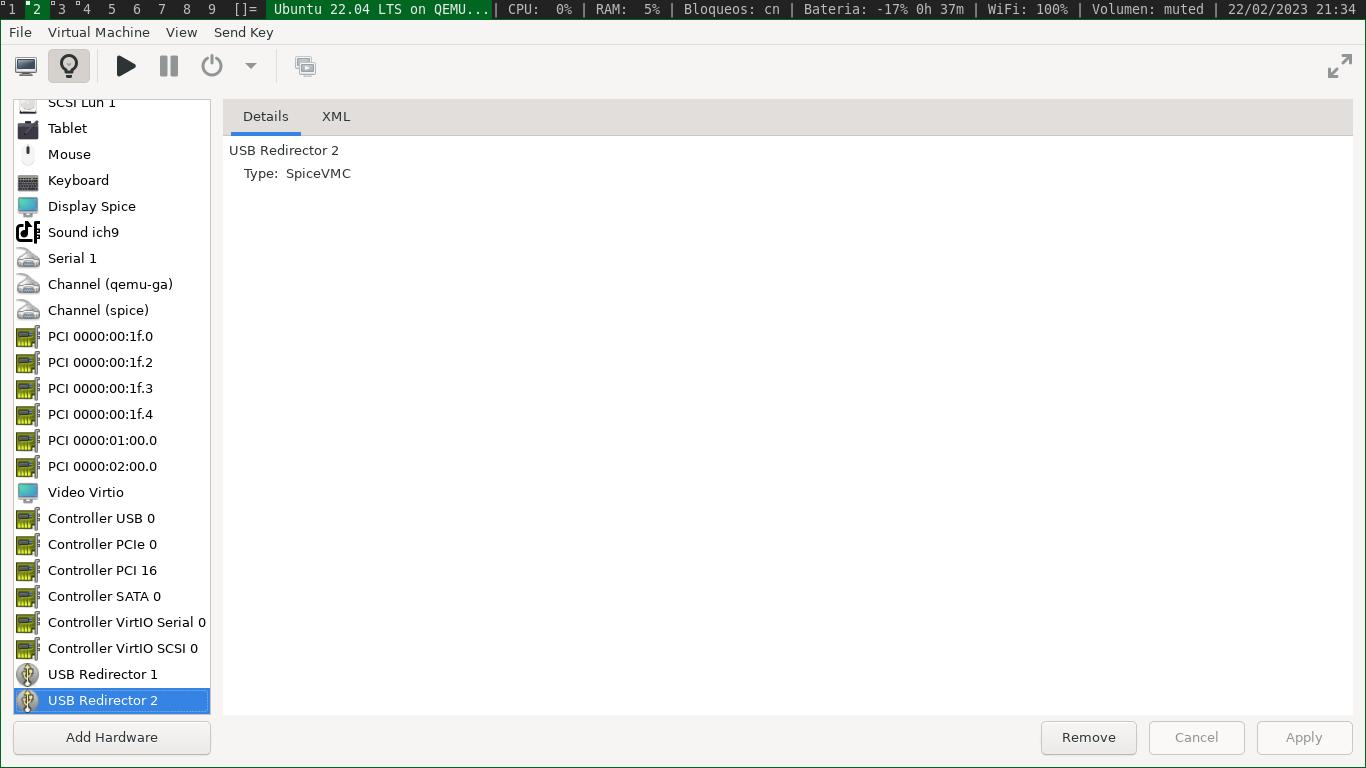
\includegraphics[width=\textwidth]{virtualMachine30}
\end{figure}
\newpage
\begin{figure}[!ht]
  \caption{Generador de números aleatorios de \acrshort{mv}}
  \centering
  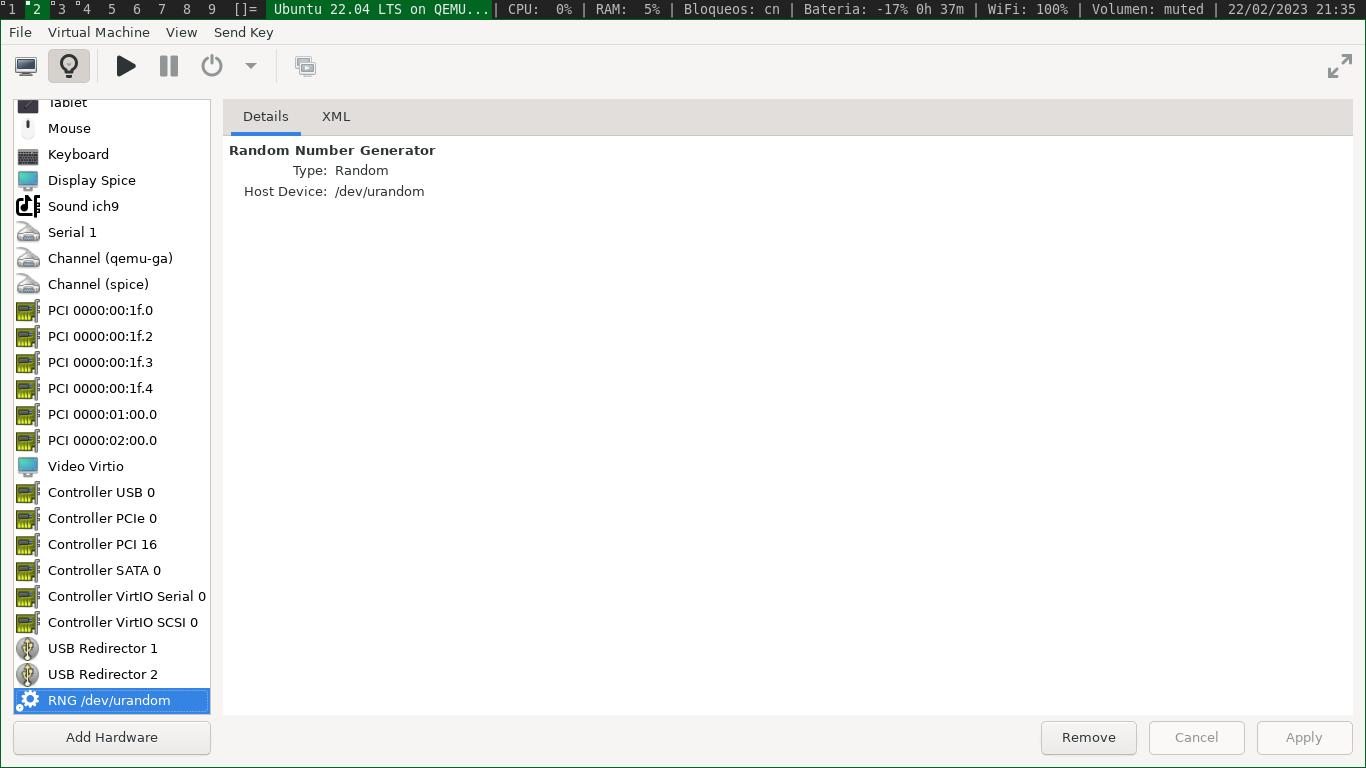
\includegraphics[width=\textwidth]{virtualMachine31}
\end{figure}
\normalsize{ \indent
Para la instalación de los paquetes de Haskell,
se utilizará el gestor de paquetes Apt; de todas
formas, es posible mejorar la experiencia de
ciertas características utilizando cabal (aunque
para lo que se realizará, no hará falta).
}
\newline
\normalsize{ \indent
Si bien, puede instalarse Termonad por el gestor
de paquetes; la única forma de que el programa
sea modificable con un archivo de Haskell es
compilando el programa (revisar
\url{https://github.com/cdepillabout/termonad#running-with-stack}),
por lo que se necesitará adicionalmente Stack
\cite{haskell_stack}.
}

	\chapter{Instrucciones}
	\normalsize{ \indent
Para instalar todos los componentes necesarios en
Ubuntu 22.04 LTS, se siguieron los siguientes pasos:
}
\begin{itemize}
	\item sudo apt install xmonad libghc-extra-dev
	\textbackslash \\ libghc-xmonad-contrib-dev
	libghc-xmonad-wallpaper-dev \textbackslash \\
	xmobar compton curl rofi scrot stterm git
	gnome-screensaver \textbackslash \\ g++ gcc
	libc6-dev libffi-dev libgmp-dev make	xz-utils
	\textbackslash \\ zlib1g-dev gnupg netbase \\
	Donde:
	\begin{itemize}
		\item xmonad es el ejecutable del gestor
		de ventanas.
		\item libghc-extra-dev provee librerías
		extras para \acrshort{ghc}, necesarias
		en el archivo xmonad.hs modificado.
		\item libghc-xmonad-contrib-dev es la
		librería de XMonad Contrib.
		\item libghc-xmonad-wallpaper-dev provee
		la función de seleccionar aleatoriamente
		el fondo de pantalla desde xmonad.hs.
		\item xmobar es el ejecutable de la barra
		de estado.
		\item compton es el \gls{comp}.
		\item curl servirá para una instrucción
		posterior.
		\item rofi es el lanzador de aplicaciones.
		\item scrot es una herramienta para
		capturar pantallas.
		\item stterm es una terminal minimalista
		que servirá para su ejecución en casos
		distintos a la principal (Termonad).
		\item git servirá para clonar el
		repositorio de una aplicación
		\item gnome-screensaver sirve para
		bloquear la pantalla en un entorno con
		\acrshort{gdm}.
		\item El resto de los paquetes
		corresponde a las dependencias dentro de
		un comando a realizar posteriormente.
	\end{itemize}
	\item curl -sSL https://get.haskellstack.org/
	| sh
	\item sudo apt install gobject-introspection
	libgirepository1.0-dev \textbackslash \\
	libgtk-3-dev libvte-2.91-dev libpcre2-dev \\
	Donde todos los paquetes son dependencias
	para poder construir Termonad.
	\item cd directorio/a/gusto
	\item git clone
	\url{https://github.com/cdepillabout/termonad}
	\item cd termonad/
	\item stack build
	\item stack run
\end{itemize}
\ \newline
\normalsize{ \indent
Posteriormente, para poder configurar de forma
correcta; es necesario recompilar todos los
archivos de Haskell, donde:
}
\begin{itemize}
	\item XMonad se compila con el comando
	``xmonad -{}-recompile'' y se reinicia con
	``xmonad -{}-restart''. Esta última acción
	afecta a XMobar, por lo que no se necesita
	más acciones para la barra de estado.
	\item Termonad se configura realizando
	``stack exec -{}-package termonad -{}-package
	colour -{}- termonad'' desde $\sim$/.local/bin.
	Adicionalmente, se copia el archivo
	$\sim$/.cache/termonad/termonad-linux-x86\textunderscore
	64 dentro del directorio /usr/local/bin
	(puede ser cualquier otro directorio
	dentro del PATH, lo único que se busca
	es evitar añadir el directorio origen
	del archivo)
\end{itemize}
\ \newline
\normalsize{ \indent
Para el caso de Rofi, no habrá necesiad de
ninguna compilación; con actualizar el
archivo $\sim$/.config/rofi/config.rasi es
suficiente, ya que el programa lee esta
configuración cada vez que se ejecuta.
}
\newline
\normalsize{ \indent
Por siguiente, para la aplicación que permite
hacer acciones sobre la sesión actual; se
clona desde el repositorio de Distrotube
\url{https://gitlab.com/dwt1/byebye}, así
se cambia lo necesario y se obtiene el
ejecutable. Dentro de lo modificado, se
encuentra la traducción de las opciones
en español y la adaptación de algunos
comandos para que funcionen en la máquina
virtual.
}
\newline
\normalsize{ \indent
Para construir la aplicación, se utiliza
``stack build'' desde el directorio en donde
se clonó el repositorio; para obtener el
ejecutable en \\
.stack-work/install/unicaCarpetaAqui/hash/version/bin/byebye-exe,
que se copia dentro de /usr/local/bin por
las mismas razones que Termonad.
}
\newline
\normalsize{ \indent
Adicionalmente, se ha ajustado la salida
de audio controlada por defecto desde
alsamixer; para ello, se ha seguido los
siguientes pasos:
}
\begin{itemize}
	\item Listar las fuentes de sonido
	con ``pactl list short sources''.
	\item Seleccionar la fuente de sonido
	correcta con ``pactl set-default-source
	nombreFuenteSonido''.
	\item Listar los disipadores de sonido
	con ``pactl list short sinks''.
	\item Seleccionar el disipador de sonido
	correcta con ``pactl set-default-sink
	nombreDisipadorSonido''.
\end{itemize}
\ \newline
\normalsize{ \indent
Con todos estos pasos realizados, se
consigue el entorno de escritorio deseado
en Ubuntu con XMonad. Para obtener las
configuraciones de cada programa y la
aplicación personalizada, se puede acceder
al siguiente repositorio:
\url{https://github.com/rodrigoantoniak/pylp}
}
	\chapter{Resultados}
	\normalsize{ \indent
Por cada área de los objetivos a abarcar,
se ha obtenido los siguientes resultados:
}
\begin{table}[ht]
\begin{center}
\begin{tabular}{ |p{2.5cm}|p{10cm}| } 
	\hline
	Menú de Inicio & Usando TreeSelect en
	XMonad, se obtiene un menú personalizado
	que otorga las opciones que se desea;
	incluyendo las esperadas en un menú
	de inicio. \\
	\hline
	Barra de Estado & XMobar es más que
	satisfactoria en la transmisión de
	información sobre el sistema. \\
	\hline
	Accesibilidad a Periféricos & Hay
	distintas formas de cubrir estas
	necesidades. Para el área de
	almacenamiento extraíble, todas
	las operaciones de un usuario
	promedio se cubren en el gestor
	de archivos Nautilus (propio de GNOME);
	si se ocupara otro que fuera gráfico,
	también cubriría esta necesidad.
	Para WiFi y salida de sonido, se
	utiliza \acrshort{tui}s para poder
	cubrir la necesidad; ejecutándose
	dentro de una terminal que se activa
	con ScratchPads. Para Bluetooth, es
	imposible inspeccionar la funcionalidad;
	considerando que no se puede trasladar
	esta capacidad a la máquina virtual,
	aunque haya formas de trabajarlo\\ 
	\hline
	Menú de acciones para la Sesión & Con
	la aplicación byebye de Derek Taylor
	(conocido en YouTube como DistroTube,
	o DT abreviadamente) y pocas
	modificaciones; se logra el objetivo,
	incluso teniendo otra forma de
	acceso a estas acciones desde el
	menú que se asemeja al menú de
	Inicio.\\ 
	\hline
\end{tabular}
\end{center}
\caption{Tabla de resultados}
\label{resultados}
\end{table}
\ \newline
\normalsize{ \indent
El único problema que se ha encontrado es
que Firefox se fuerza a ir para el tercer
espacio de trabajo, lo cual puede ser un
error propio de XMonad o porque el archivo
binario utilizado conserva la memoria de
lo usado por defecto; más allá de eso,
no se ha encontrado fallas.
}
\newline
\normalsize{ \indent
A continuación, se mostrará algunas
capturas del entorno de escritorio
resultante:
}
\newpage
\begin{figure}[!ht]
  \caption{Primera captura de \acrshort{mv}}
  \centering
  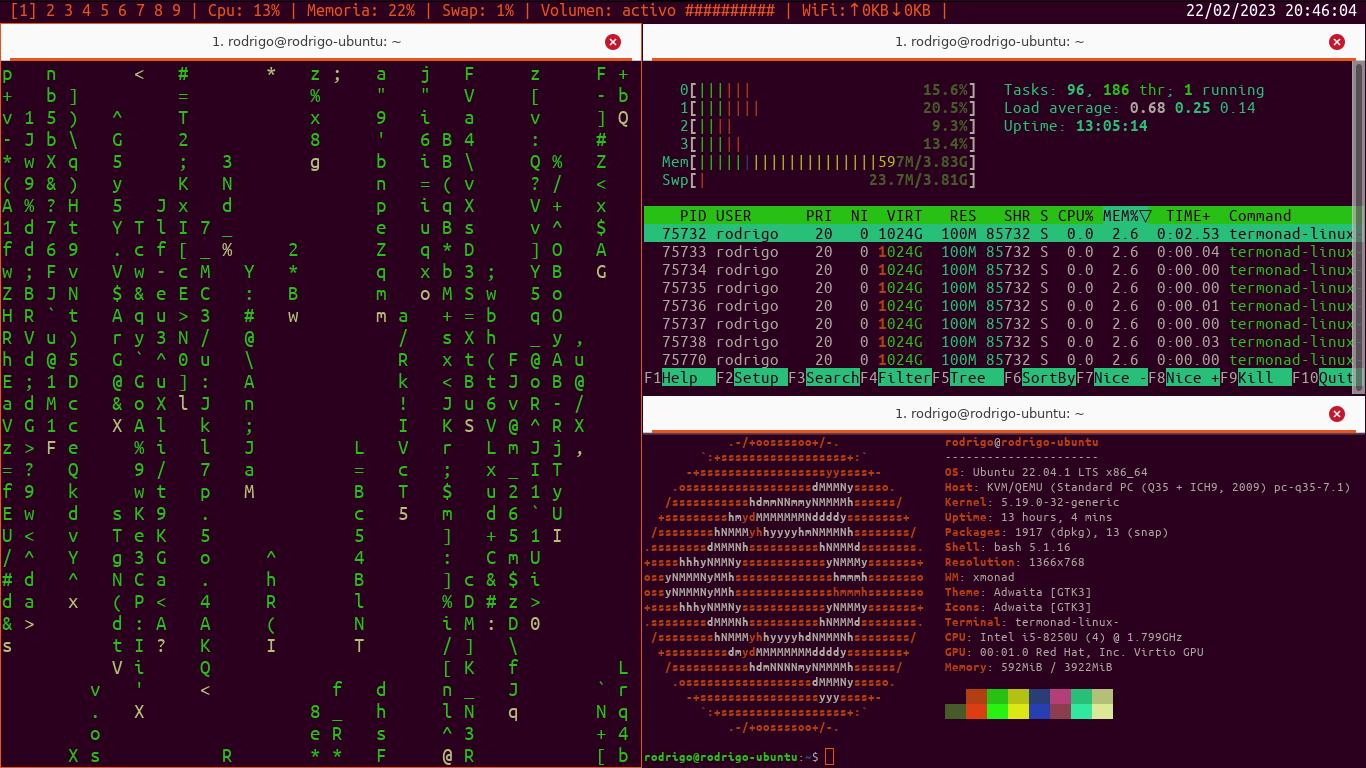
\includegraphics[width=\textwidth]{resultado1}
\end{figure}
\begin{figure}[!ht]
  \caption{Segunda captura de \acrshort{mv}}
  \centering
  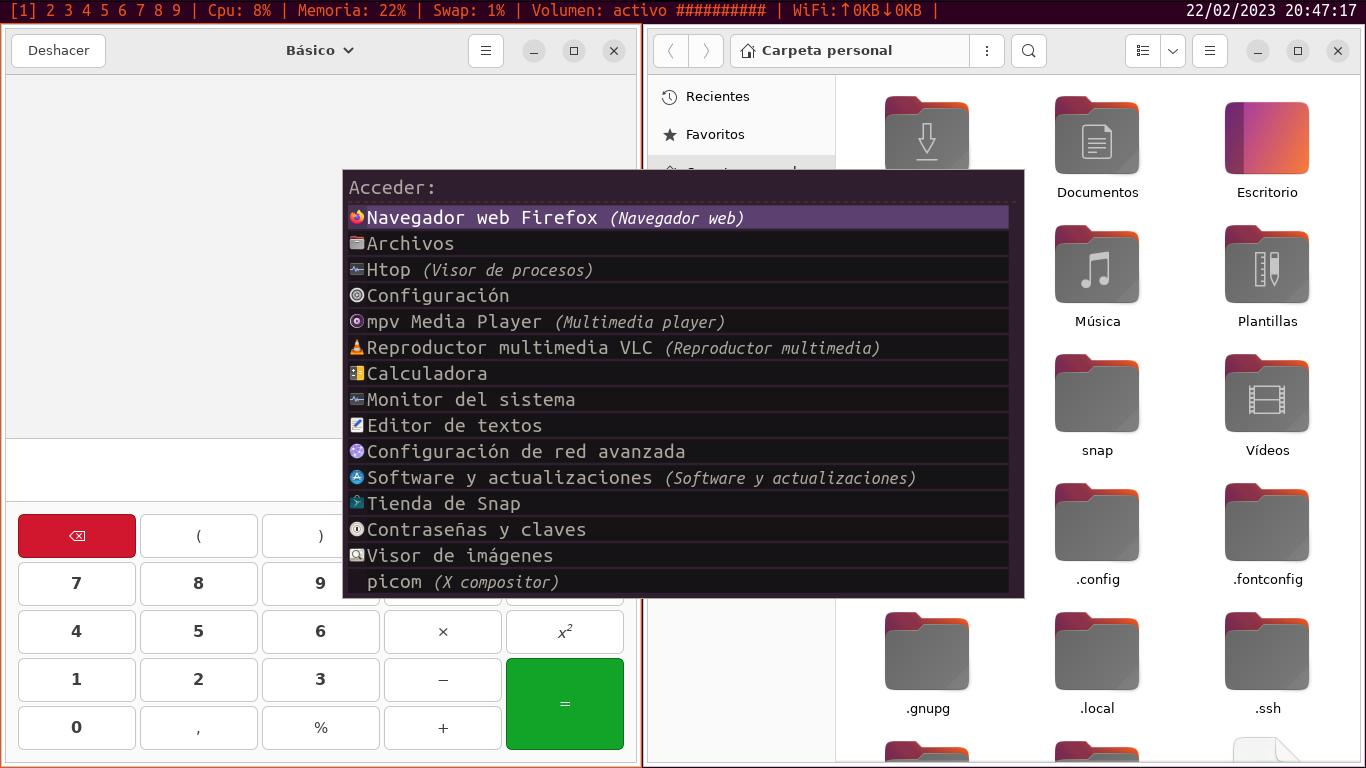
\includegraphics[width=\textwidth]{resultado2}
\end{figure}
\newpage
\begin{figure}[!ht]
  \caption{Tercera captura de \acrshort{mv}}
  \centering
  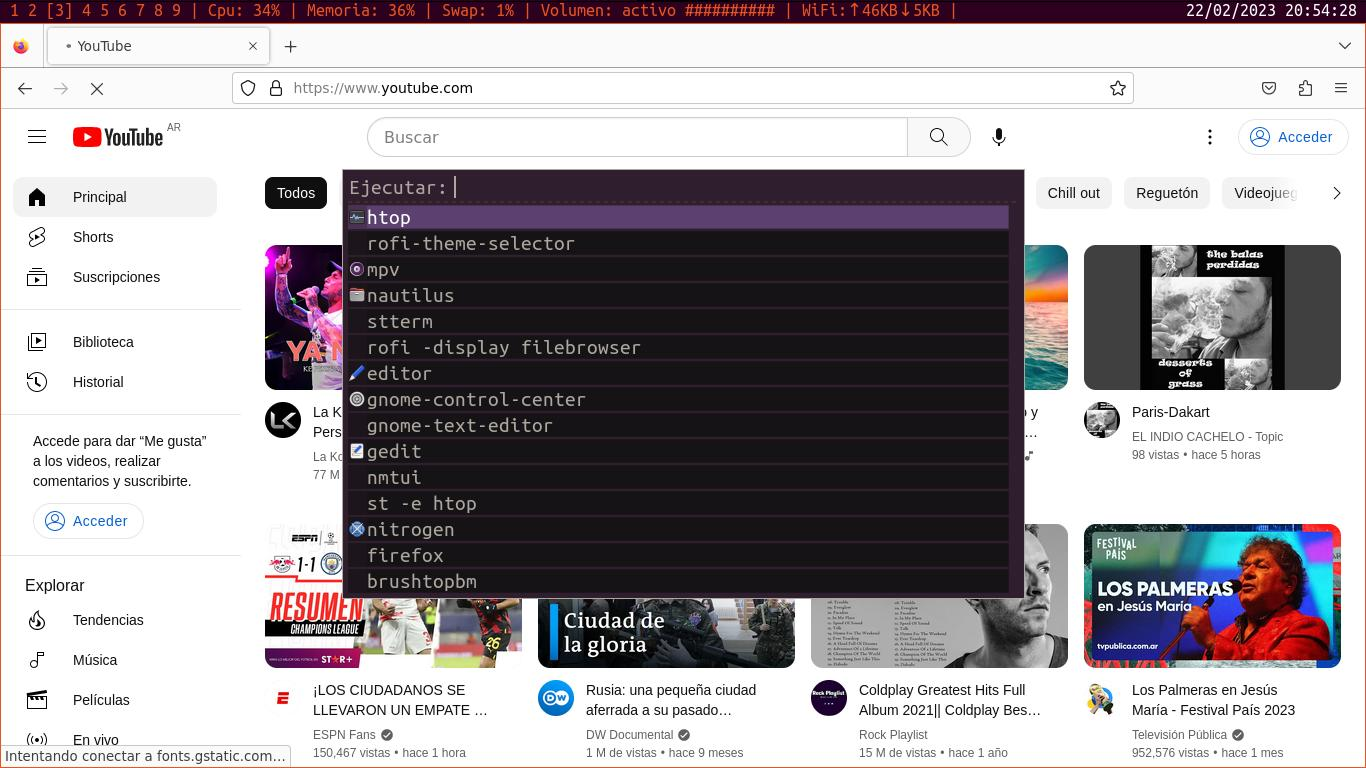
\includegraphics[width=\textwidth]{resultado3}
\end{figure}
\begin{figure}[!ht]
  \caption{Cuarta captura de \acrshort{mv}}
  \centering
  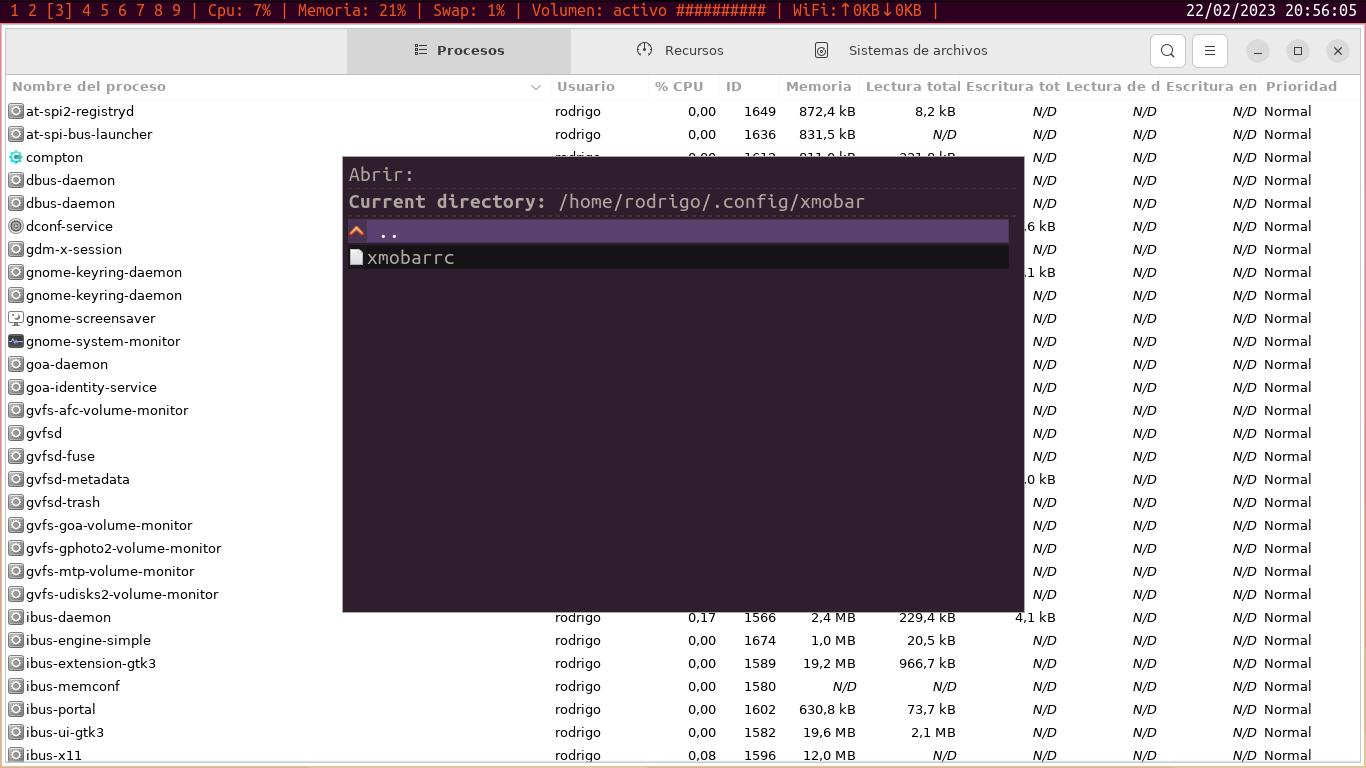
\includegraphics[width=\textwidth]{resultado4}
\end{figure}
\newpage
\begin{figure}[!ht]
  \caption{Quinta captura de \acrshort{mv}}
  \centering
  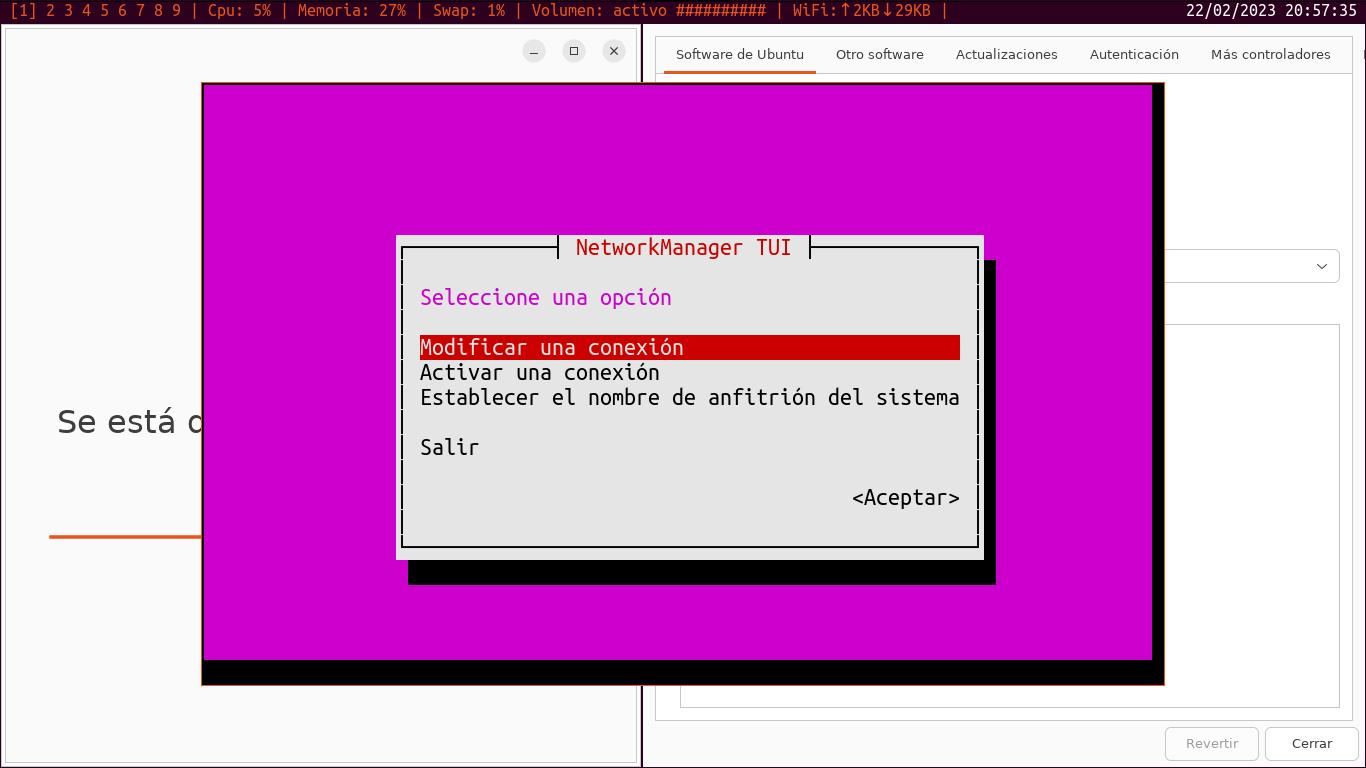
\includegraphics[width=\textwidth]{resultado5}
\end{figure}
\begin{figure}[!ht]
  \caption{Sexta captura de \acrshort{mv}}
  \centering
  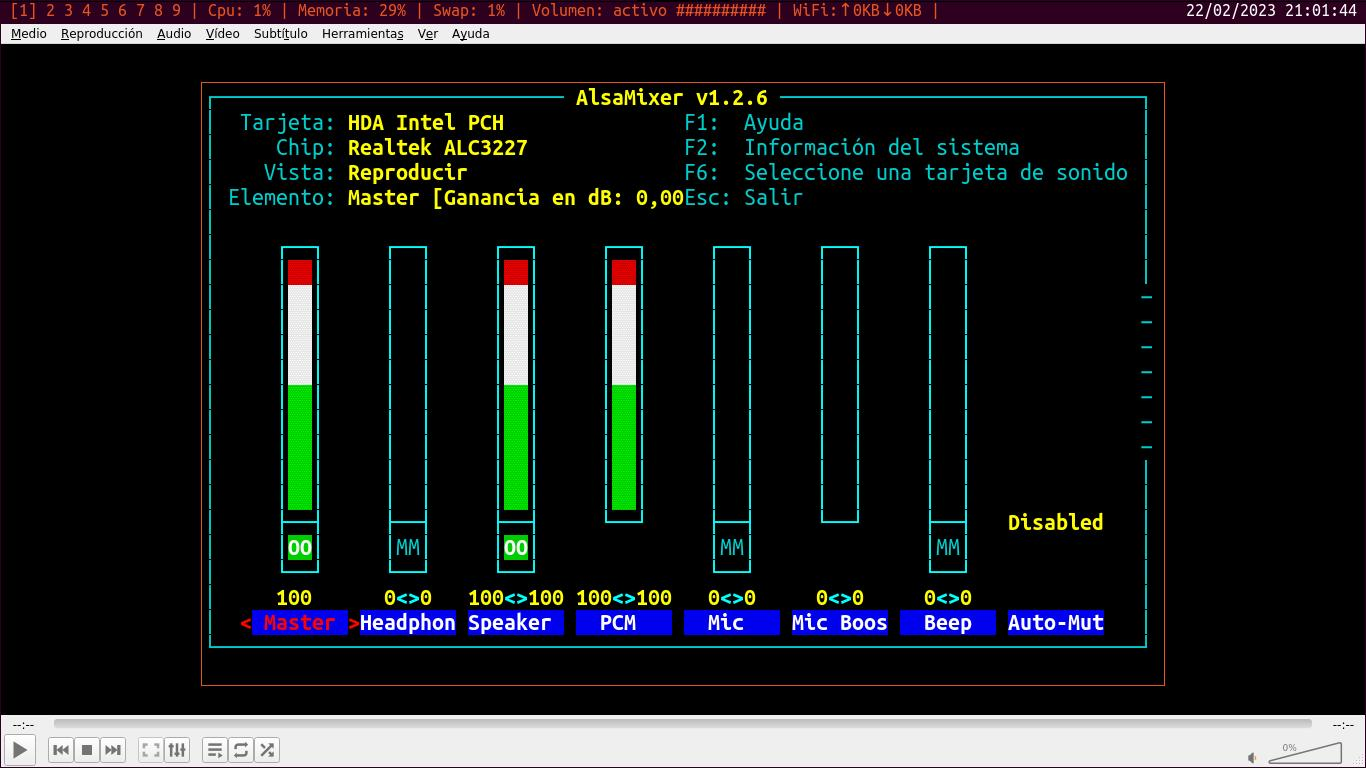
\includegraphics[width=\textwidth]{resultado6}
\end{figure}
\newpage
\begin{figure}[!ht]
  \caption{Séptima captura de \acrshort{mv}}
  \centering
  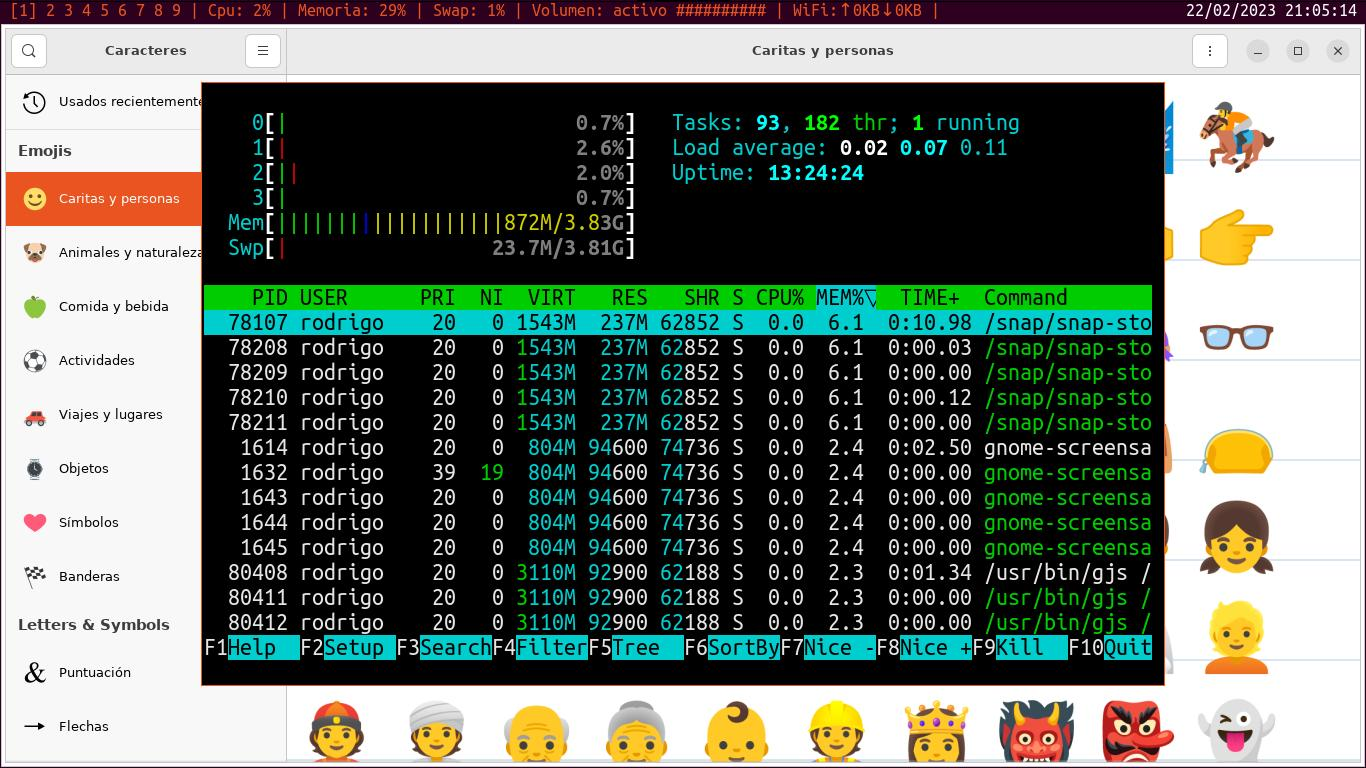
\includegraphics[width=\textwidth]{resultado7}
\end{figure}
\begin{figure}[!ht]
  \caption{Octava captura de \acrshort{mv}}
  \centering
  
\includegraphics[width=\textwidth]{resultado8}
\end{figure}
\newpage
\begin{figure}[!ht]
  \caption{Novena captura de \acrshort{mv}}
  \centering
  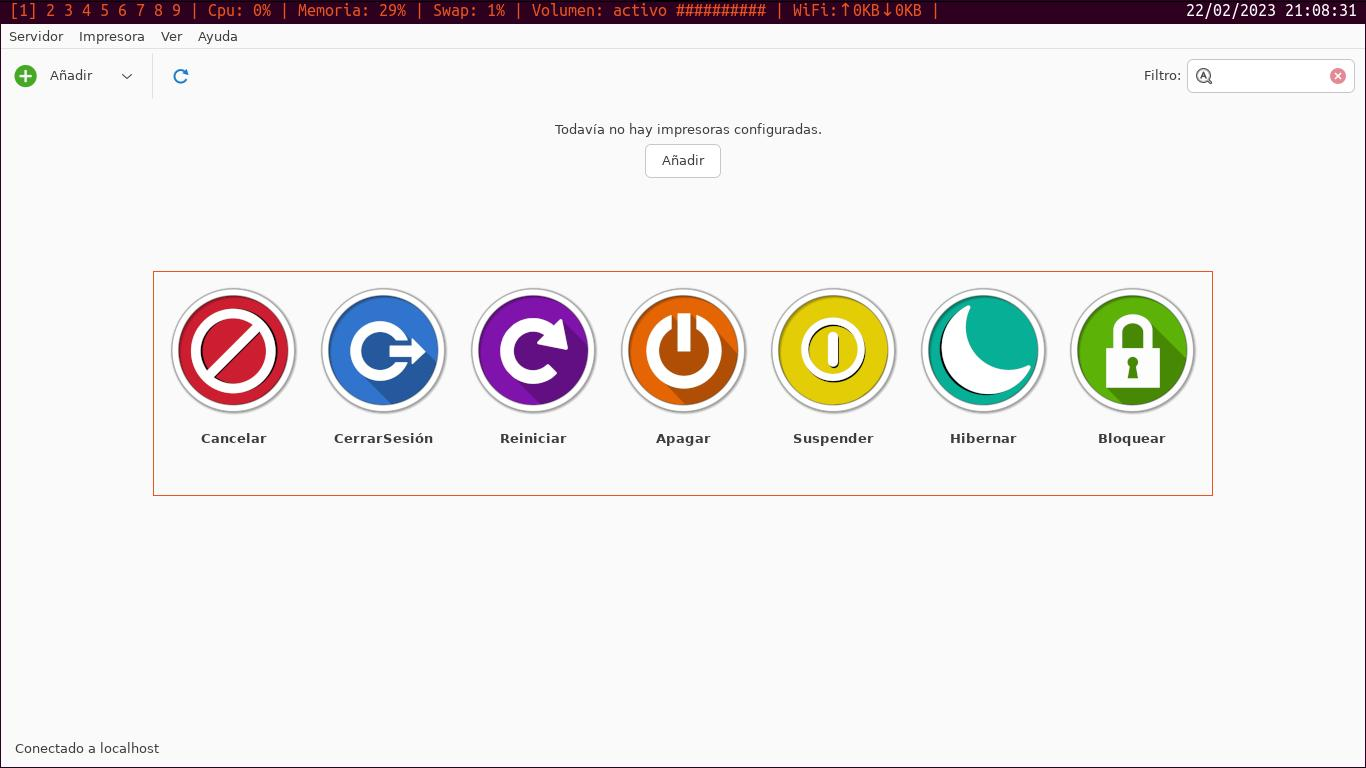
\includegraphics[width=\textwidth]{resultado9}
\end{figure}
	\appendix
	\chapter[Glosario]{Glosario de Términos}
	\printnoidxglossary[type=\acronymtype,
    		title=Abreviaturas y acrónimos,nonumberlist]
	\printnoidxglossary[title=Definiciones,nonumberlist]
	\backmatter
	\chapter[Bibliografía]{Referencias
		bibliográficas}
	\printbibliography
\end{document}
